% -----------------------------------------------------------------------
% IEEE Transactions on Industrial Informatics — journal submission
% -----------------------------------------------------------------------
\documentclass[journal]{IEEEtran}

\usepackage[T1]{fontenc}
\usepackage[utf8]{inputenc}
\usepackage{amsmath,amssymb}
\usepackage{graphicx}
\usepackage{booktabs}
\usepackage{siunitx}
\usepackage{array}
\usepackage{xcolor}
\usepackage{algorithm}
\usepackage{algpseudocode}
\usepackage{tikz}
\usepackage{pgfplots}
\pgfplotsset{compat=1.18}
\usepackage{cite}
\usepackage{url}
\usepackage{microtype}

\usetikzlibrary{shapes.geometric, arrows.meta, positioning, fit,
                backgrounds, decorations.pathreplacing, calc,
                patterns}

% -----------------------------------------------------------------------
\begin{document}

\title{TRAW: Traffic-Aware Multi-Pass RAW Scheduling\\
for Dense IEEE~802.11ah Industrial IoT Networks}

\author{Alakesh~Kalita,~\IEEEmembership{Senior~Member,~IEEE,}
        and~Nurzaman~Ahmed,~\IEEEmembership{Member,~IEEE}%
\thanks{Both authors are with the Department of Mathematics
and Computing, Indian Institute of Technology (ISM) Dhanbad,
India (e-mail: \{alakesh.kalita1025, nurzaman713\}@gmail.com).}%
\thanks{Manuscript received --; revised --; accepted --.}}

\markboth{IEEE Transactions on Industrial Informatics,~Vol.~XX,
No.~X, Month~20XX}%
{Kalita and Ahmed: TRAW for Dense IEEE 802.11ah IIoT Networks}

\IEEEpeerreviewmaketitle

% -----------------------------------------------------------------------
\begin{abstract}
IEEE~802.11ah enables large-scale sub-1-GHz wireless connectivity for
Industrial Internet of Things (IIoT) deployments through the Restricted
Access Window (RAW) mechanism. However, existing RAW schedulers often
allocate access opportunities uniformly, which limits their ability to
serve bursty sensor groups while conserving energy for idle devices. To
address this problem, this paper proposes traffic-aware RAW (TRAW), a
standards-compatible AP-side scheduler for dense IEEE~802.11ah IIoT
networks. TRAW combines CUSUM-boosted EWMA demand estimation with
demand-proportional slot allocation, multi-pass RAW scheduling for
overloaded groups, and PRAW-style idle-group suspension. It also
introduces a target-slot group initialization rule and a budget-safe
split feasibility check to avoid over-fragmentation and structural
freeze under congestion. We evaluate TRAW in an IEEE~802.11ah simulator
for $100$--$1000$ stations over multiple random seeds. Compared with
the strongest baseline, TRAW improves packet delivery ratio by up to
15.8\%, reduces mean delay by up to 15.0\%, lowers deadline violation
rate by up to 4.4\%, and improves energy efficiency by up to 12.9\%
under heavy load. The results also reveal a clear trade-off: finer RAW
partitioning improves throughput and delay, but can slightly increase
Age of Information and association latency.
\end{abstract}

\begin{IEEEkeywords}
IEEE 802.11ah, Wi-Fi HaLow, industrial IoT, restricted access window,
PRAW, multi-pass scheduling, Age of Information, demand-proportional
allocation, CUSUM-EWMA, dense IoT, beacon scheduling, Industry~4.0.
\end{IEEEkeywords}

% -----------------------------------------------------------------------
\section{Introduction}
\label{sec:intro}

\IEEEPARstart{T}{he} Industrial Internet of Things (IIoT) is increasingly
used for smart manufacturing, predictive maintenance, factory
automation, and process monitoring. A single production floor can
include hundreds or thousands of sensors that periodically report
vibration, temperature, pressure, current, occupancy, and environmental
measurements to a gateway. Such networks are difficult to support using
conventional contention-based access because they combine high station
density, strict delay and freshness requirements, and long battery
lifetime expectations~\cite{chen2017iiot,Sisinni2018}.

IEEE~802.11ah, also known as Wi-Fi HaLow, was introduced for long-range
and low-power wireless access below 1~GHz~\cite{std80211ah}. It supports
large basic service sets and provides several mechanisms useful for
dense IoT, including hierarchical association identifiers, beacon-based
power saving, target wake time, and the Restricted Access Window (RAW).
In RAW, the access point (AP) divides the post-beacon contention period
into group-specific access windows. Stations whose association
identifiers fall inside a configured group contend only in their
assigned RAW slots. This reduces the number of simultaneous contenders
and improves scalability in dense deployments.

However, RAW performance depends strongly on how the AP forms groups,
assigns slot counts, and chooses slot durations. A static RAW
configuration can be efficient under stable traffic, but it wastes
airtime when groups are idle and becomes insufficient when correlated
industrial events create bursts. Existing adaptive RAW policies improve
this behavior, but they commonly retain three limitations. First, groups
are often treated uniformly even when their instantaneous traffic
demands differ. Second, a congested group normally receives only one RAW
opportunity in a beacon interval. Third, split decisions can become
blocked under heavy backlog when feasibility is evaluated using the
backlog-inflated slot duration rather than the physical minimum feasible
duration. These limitations motivate a RAW scheduler that can reallocate
airtime toward busy groups while preserving a safe minimum service level
for all active groups.

To address the above issues, this paper proposes traffic-aware RAW
(TRAW), an AP-side scheduling framework for dense IEEE~802.11ah IIoT
networks. TRAW is designed using RAW/RPS primitives available in
IEEE~802.11ah and is evaluated as a simulator-level standards-compatible
scheduler. The current implementation uses simulator-visible station
queue occupancy as an ideal demand signal; a deployable implementation
can replace this signal with AP-observable buffer status, uplink
history, missed-report counters, or application-layer queue reports.
This distinction is stated explicitly because the objective of this work
is to quantify the performance potential of traffic-aware RAW scheduling
under transparent assumptions, not to introduce a new PHY/MAC frame
format.

The main contributions of this article are as follows.
\begin{enumerate}
  \item We propose a CUSUM-boosted EWMA demand estimator that captures
        both persistent traffic load and sudden burst growth in each
        station group.
  \item We design a floor-protected demand-proportional allocation
        method that redistributes RAW slot opportunities from
        low-demand groups to high-demand groups without starving
        lightly loaded groups.
  \item We introduce a multi-pass RAW scheduling mechanism in which
        overloaded groups may receive a second non-overlapping RAW
        opportunity within the same beacon interval.
  \item We incorporate PRAW-style idle-group suspension so that groups
        with sustained near-zero demand are scheduled only
        periodically, releasing airtime for active groups.
  \item We add two architectural safeguards: target-slot group
        initialization to avoid excessive fragmentation at startup, and
        budget-safe split feasibility based on the minimum RAW slot
        duration to prevent structural freeze during congestion.
  \item We evaluate TRAW against No-RAW, Static RAW, Adaptive RAW,
        LACA, Chang2019, and TASM-RAW for $N\!\in\!\{100,\ldots,1000\}$
        stations.
        The results show up to 15.8\% higher packet delivery ratio,
        15.0\% lower mean delay, 4.4\% lower deadline violation rate,
        and 12.9\% higher energy efficiency than the strongest baseline
        under heavy load.
\end{enumerate}

A key finding is that TRAW is not uniformly superior on every metric.
Its finer 37-group partition improves throughput, delay, and energy
efficiency, but it can slightly increase mean Age of Information and
association latency because each group recurs less frequently than in
the 32-group TASM-RAW baseline. This trade-off is analyzed explicitly in
Section~\ref{sec:assoc-tradeoff} and leads to deployment guidelines in
Section~\ref{sec:discuss}.

The rest of this article is organized as follows. Section~\ref{sec:related}
reviews related work. Section~\ref{sec:model} describes the system model
and performance requirements. Section~\ref{sec:design} presents the TRAW
algorithm. Section~\ref{sec:eval} reports simulation results.
Section~\ref{sec:discuss} discusses deployment guidelines, and
Section~\ref{sec:conc} concludes the article.

% -----------------------------------------------------------------------
\section{Related Work}
\label{sec:related}

\subsection{IIoT Wireless Connectivity}

Early IIoT deployments relied on WirelessHART and ISA100.11a
(2.4\,GHz DSSS mesh), which provide high reliability via source-routing
and time-division access but support at most a few hundred nodes per
network~\cite{chen2017iiot}.
LoRa and Sigfox achieve km-range coverage at sub-kb/s rates but are
unsuitable for periodic high-frequency reporting because duty-cycle
regulations restrict throughput to a few hundred bytes per hour.
IEEE~802.11ah fills the gap: it provides sub-GHz penetration, 150--7800\,kb/s
data rates, and 8191-station BSS capacity, with the RAW mechanism
ensuring scalable channel access~\cite{Sisinni2018}.

\subsection{RAW Performance Analysis}

Tian et al.~\cite{tian2016} derive closed-form optimal group count and
slot duration for static saturated traffic using Markov chain analysis.
Raeesi et al.~\cite{raeesi2014} show that static RAW outperforms plain
CSMA-CA beyond $N\!=\!50$ but degrades sharply when provisioned group
sizes mismatch actual station count.
Both analyses assume fixed traffic and cannot respond to load changes
within a running deployment.

\subsection{Adaptive Slot Sizing}

Kim et al.~\cite{kim2017raw} adjust the RAW slot duration based on
estimated collision probability, reducing overhead for lightly-loaded
groups.
Bhandari and Moh~\cite{bhandari2018} propose a priority-based adaptive
MAC that modifies slot duration via collision feedback.
Taramit et al.~\cite{taramit2023} introduce LACA, a renewal-process
model that computes optimal slot duration T* for a single fixed group
as the expected time for $n_s$ sequential deliveries; TRAW extends this
model across dynamically-sized groups.
Kalita and Ahmed~\cite{kalita2025} add CUSUM detection to EWMA smoothing
for faster response to sustained load increases; TRAW inherits this
estimator and extends it to drive multi-pass scheduling decisions.

\subsection{Dynamic Grouping}

Kim and Moh~\cite{kim2017} assign RAW groups based on pre-provisioned
cluster membership, which does not adapt to runtime demand shifts.
Chang et al.~\cite{chang2019} collect per-STA demand reports via
management frames to drive group reassignment; the overhead is
incompatible with battery-constrained IIoT nodes.
Kalita and Ahmed~\cite{kalita2025b} (TASM-RAW) combine CUSUM-EWMA
prediction with load-median split/merge and budget-aware group count
to adapt $G$ and $\{D_g\}$ per beacon without station feedback; TRAW
extends this foundation with mechanisms A, B, and C.

\subsection{PRAW and Energy-Aware Scheduling}

The PRAW element (Section~9.4.2.200~\cite{std80211ah}) is specified for
static provisioning of infrequent sensor groups at deployment time.
Park and Hwang~\cite{park2019praw} study PRAW performance under
homogeneous Poisson traffic but do not provide adaptive period selection.
To our knowledge, no prior work dynamically assigns PRAW mode to
individual groups based on live per-beacon demand estimates.

\subsection{Age of Information for IIoT}

AoI was introduced by Kaul et al.~\cite{kaul2012aoi} as a metric for
information freshness.
Subsequent work~\cite{yates2021aoi} characterises AoI for a variety
of queuing models.
Abd-Elmagid et al.~\cite{abdelmagid2019aoi} study AoI under energy
harvesting constraints.
In the 802.11ah context, the impact of RAW slot allocation on AoI
has not been studied; we provide the first analysis relating
demand-proportional RAW allocation to mean AoI.

% -----------------------------------------------------------------------
\section{IIoT System Model}
\label{sec:model}

\subsection{Network Topology and PHY}

We model a single-cell star BSS with one AP serving $N$ uplink STAs,
representative of an industrial gateway serving a factory floor zone.
All nodes use the lowest 1\,MHz S1G data rate, 150\,kb/s
(BPSK~$\frac{1}{2}$, referred to as MCS10 in the 2$\times$-repetition
1\,MHz mode of the IEEE~802.11ah amendment; we retain the simulator's
internal label ``MCS0'' for this rate throughout, and note that some
implementation guides instead use ``MCS0'' for the 300\,kb/s
non-repeated 1\,MHz rate)\footnote{The simulator's PHY mode table maps
the label \texttt{MCS0} to 150\,kb/s for all numerical results in this
paper (\texttt{sim11ah/config.py}); this is the conservative,
lowest-rate 1\,MHz S1G mode irrespective of the MCS-index naming
convention used.} on a 915\,MHz
channel with AWGN path loss appropriate for sub-GHz indoor industrial
propagation.
The AP broadcasts a DTIM beacon every $T_B\!=\!500$\,ms.
Each beacon carries a RAW Parameter Set (RPS) element that partitions
AIDs $\{1,\ldots,N\}$ into $G(t)$ non-overlapping groups
$\mathcal{G}(t)=\{[s_1,e_1],\ldots,[s_G,e_G]\}$; each group $g$
receives a window of $S_g(t)$ sub-slots each of duration $D_g(t)$.
STAs transmit only during their assigned window; during all other
windows they enter deep sleep, saving battery power.

\subsection{Industrial Traffic Model}

IIoT sensors exhibit a two-mode traffic pattern:

\textbf{Quiescent mode.}
Sensors report a single uplink packet (128\,bytes, MCS0) every
$T_\mathrm{rep}\!=\!5$\,s, covering periodic machine health telemetry,
environmental sensing, and asset-tracking pings.
This generates a per-STA MAC queue depth of approximately 0.1 packets
per 500\,ms beacon interval, equivalent to per-AID demand
$\lambda_i\!\approx\!0.1$.

\textbf{Burst mode.}
A production anomaly (bearing failure, temperature spike, flow deviation)
causes all sensors in an affected machine zone to sample at 1\,Hz for
the duration of the event.
In a typical 25-STA group this raises per-AID demand to
$\lambda_g\!\approx\!1\!-\!2$, saturating the single-window RAW
allocation and requiring either larger slots or additional windows.
The CUSUM component of TRAW's estimator is designed to detect this
transition within 2--3 beacon intervals.

\textbf{Idle mode.}
Battery-powered sensors with long reporting periods (asset tags,
once-per-minute gas sensors) may generate fewer than 0.01 packets per BI
for tens of seconds at a time.
The PRAW mechanism in TRAW suppresses these groups to 1-of-4 beacons
after 65\,s of confirmed silence, extending battery life proportionally.

\subsection{Industrial Performance Requirements}

We target three metrics relevant to industrial deployments:

\textbf{Packet delivery ratio (PDR).}
Safety-critical monitoring (emergency stop, overpressure) requires
PDR\,$\geq$\,0.99; condition monitoring tolerates PDR\,$\geq$\,0.95;
environmental sensing accepts PDR\,$\geq$\,0.80~\cite{Sisinni2018}.

\textbf{Mean Age of Information (AoI).}
For a sensor with reporting period $T_\mathrm{rep}$ and delivery
probability $p$ per period, the steady-state mean AoI is
\begin{equation}
  \overline{\Delta} = T_\mathrm{rep}\cdot\frac{2-p}{2p},
  \label{eq:aoi}
\end{equation}
obtained by modelling successful updates as a geometric renewal process.
For $T_\mathrm{rep}\!=\!5$\,s:
at $p\!=\!1$, $\overline{\Delta}\!=\!2.5$\,s (one half-period);
at $p\!=\!0.5$, $\overline{\Delta}\!=\!7.5$\,s (three half-periods).
In this paper we \emph{adopt} $\overline{\Delta}\!\leq\!3T_\mathrm{rep}$
(stale data no older than three reporting cycles) as a representative
design target for condition-monitoring applications, consistent with
the periodic-reporting freshness budgets discussed in
\cite{Sisinni2018}; we do not claim this threshold as a universal
industrial requirement, and deployments with tighter or looser
freshness needs should rescale the bound accordingly.

\textbf{Deadline Violation Rate (DVR).}
DVR is the fraction of generated packets not delivered within the
reporting cycle, approximated as $\mathrm{DVR}\!\approx\!1\!-\!\mathrm{PDR}$
when the MAC TX queue flushes each cycle's packet on the next
generation event~\cite{Sisinni2018}.

\subsection{Design Objective}

At each beacon epoch $t$ choose partition $\mathcal{G}(t)$, sub-slot
counts $\{S_g(t)\}$, slot durations $\{D_g(t)\}$, and per-group PRAW
phases to minimise $\overline{\Delta}$ subject to the beacon-budget
feasibility constraint
\begin{equation}
  \sum_{g=1}^{G(t)} S_g(t)\cdot D_g(t) \;\leq\; \eta\,T_B,
  \label{eq:feasibility}
\end{equation}
where $\eta\!=\!0.90$ reserves 10\,\% for beacon overhead and initial
backoff.

% -----------------------------------------------------------------------
\section{TRAW Algorithm}
\label{sec:design}

Fig.~\ref{fig:arch} shows the per-beacon execution flow.
At each beacon epoch the AP performs seven sequential steps.
Steps~1--2 are shared with TASM-RAW~\cite{kalita2025b}; steps~3--7 are
TRAW's new contributions.

\begin{figure}[!t]
\centering
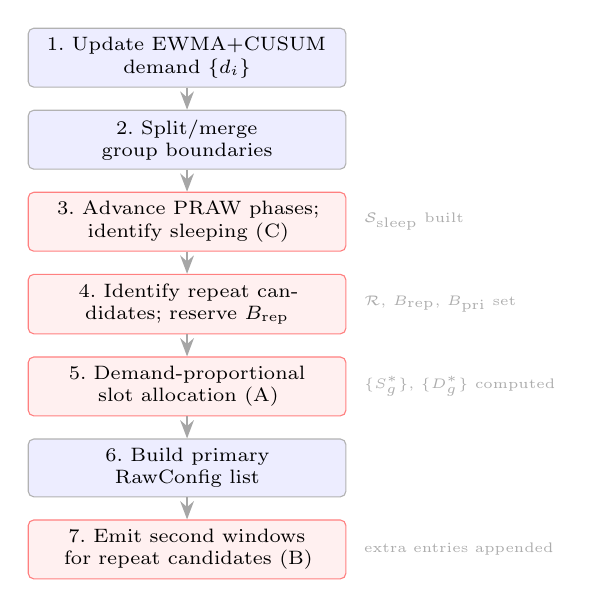
\begin{tikzpicture}[
  font=\scriptsize,
  node distance=0.28cm,
  box/.style={rectangle, rounded corners=2pt, draw=gray!60,
              fill=blue!7, minimum width=4.0cm, align=center,
              minimum height=0.52cm, text width=3.8cm},
  new/.style={rectangle, rounded corners=2pt, draw=red!50,
              fill=red!6, minimum width=4.0cm, align=center,
              minimum height=0.52cm, text width=3.8cm},
  arr/.style={->, >=Stealth, thick, gray!70},
]
  \node[box] (s1) {1.\ Update EWMA+CUSUM demand $\{d_i\}$};
  \node[box, below=of s1] (s2) {2.\ Split/merge group boundaries};
  \node[new, below=of s2] (s3) {3.\ Advance PRAW phases; identify sleeping (C)};
  \node[new, below=of s3] (s4) {4.\ Identify repeat candidates; reserve $B_\mathrm{rep}$};
  \node[new, below=of s4] (s5) {5.\ Demand-proportional slot allocation (A)};
  \node[box, below=of s5] (s6) {6.\ Build primary RawConfig list};
  \node[new, below=of s6] (s7) {7.\ Emit second windows for repeat candidates (B)};

  \draw[arr] (s1)--(s2); \draw[arr] (s2)--(s3);
  \draw[arr] (s3)--(s4); \draw[arr] (s4)--(s5);
  \draw[arr] (s5)--(s6); \draw[arr] (s6)--(s7);

  \node[right=0.1cm of s3, font=\tiny, text=gray!65, align=left]
    {$\mathcal{S}_\mathrm{sleep}$ built};
  \node[right=0.1cm of s4, font=\tiny, text=gray!65, align=left]
    {$\mathcal{R}$, $B_\mathrm{rep}$, $B_\mathrm{pri}$ set};
  \node[right=0.1cm of s5, font=\tiny, text=gray!65, align=left]
    {$\{S_g^*\}$, $\{D_g^*\}$ computed};
  \node[right=0.1cm of s7, font=\tiny, text=gray!65, align=left]
    {extra entries appended};
\end{tikzpicture}
\caption{TRAW per-beacon flow. Blue boxes (steps~1,~2,~6) are inherited
from TASM-RAW; red boxes (steps~3--5,~7) are new mechanisms.}
\label{fig:arch}
\end{figure}

% ---------
\subsection{Traffic Demand Estimation}
\label{sec:demand}

The AP maintains a per-STA queue-occupancy estimate $q_i(t)$ at each
beacon epoch $t$.
In a deployed IEEE~802.11ah network this estimate is
\emph{AP-observable}: it is computed from quantities the AP can
directly measure without relying on any STA-side cooperation beyond
what the standard already provides, namely
(i) the More Data subfield and Buffer Status Report (BSR, IEEE~802.11
Section~9.2.4.5.5/Section~9.4.1.55) carried in the most recent uplink frame from
STA~$i$, which gives an explicit (quantised) queue-length report;
(ii) the elapsed time since STA~$i$'s last successful uplink delivery
relative to its known/learned reporting period $T_\mathrm{rep},_i$,
used to flag a missed report; and
(iii) the AP's own record of how many RAW opportunities STA~$i$ was
given versus how many it used.
$q_i(t)$ is formed by combining the BSR value (when present) with a
missed-report counter that increments $q_i(t)$ by one whenever a STA's
expected reporting interval elapses without a delivered packet.
\emph{Evaluation note:} the simulation results in
Section~\ref{sec:eval} compute $q_i(t)$ directly from the simulator's
internal per-STA MAC transmit-queue length, which is equivalent to an
\emph{ideal, zero-quantisation, zero-delay BSR}.
This represents a best-case upper bound on the accuracy of the
AP-observable estimator described above; Section~\ref{sec:discuss}
discusses the expected impact of BSR quantisation and reporting delay
on the mechanisms below.

An EWMA smoother tracks the running mean:
\begin{equation}
  \hat{q}_i(t) = \alpha\,q_i(t) + (1-\alpha)\,\hat{q}_i(t-1),
  \quad \alpha=0.3.
  \label{eq:ewma}
\end{equation}
A one-sided CUSUM detects sustained increases in queue depth above the
EWMA baseline, capturing the onset of machine anomaly bursts:
\begin{align}
  e_i(t)  &= q_i(t) - \hat{q}_i(t-1), \label{eq:err}\\
  C_i(t)  &= \max\!\bigl(0,\;C_i(t-1)+e_i(t)-k\bigr),\quad k=0.15.
  \label{eq:cusum}
\end{align}
The composite demand estimate that feeds all downstream decisions is:
\begin{equation}
  d_i(t) = \max\!\bigl(0,\;\hat{q}_i(t)+\max(0,\,C_i(t)-h)\bigr),
  \quad h=0.8.
  \label{eq:demand}
\end{equation}
The slack $k$ absorbs isolated measurement noise; the threshold $h$
ensures the CUSUM boost activates only after the queue has been
persistently elevated, providing IIoT-appropriate burst discrimination.
Per-group aggregate load and normalised per-AID demand follow as:
\begin{equation}
  D_g(t) = \sum_{i=s_g}^{e_g} d_i(t), \quad
  \lambda_g(t) = \frac{D_g(t)}{e_g - s_g + 1}.
  \label{eq:groupload}
\end{equation}

% ---------
\subsection{Group Initialisation, Split, and Merge}
\label{sec:split_merge}

\textbf{Initial group count.}
At startup, TRAW bounds the group count with a target-slots criterion:
\begin{equation}
  G_\mathrm{max} = \min\!\left(
    \left\lfloor\frac{\eta\,T_B}{S_\mathrm{tgt}\cdot D_\mathrm{min}}\right\rfloor,\;
    \left\lfloor\frac{N}{n_\mathrm{min}}\right\rfloor
  \right),
  \label{eq:gmax}
\end{equation}
where $S_\mathrm{tgt}$ is the target sub-slot count (configurable via
\texttt{raw\_num\_slots}; the code default absent this override is 4,
but the evaluation in Section~\ref{sec:eval} sets
$S_\mathrm{tgt}\!=\!8$ throughout, see Table~\ref{tab:simparams}),
$D_\mathrm{min}\!\approx\!12{,}020\,\mu$s
is the minimum achievable slot duration (one complete DATA+ACK exchange
at MCS0 with mean backoff), and $n_\mathrm{min}\!=\!5$ prevents
degenerate micro-groups.
For $T_B\!=\!500$\,ms and the evaluation setting $S_\mathrm{tgt}\!=\!8$:
$G_\mathrm{max}\!=\!4$ at $N\!=\!400$, giving groups of $\sim$100 AIDs
with $S\!=\!8$ initial sub-slots each (this initial count is
independent of the 37-group \emph{steady-state} cap of
Section~\ref{sec:scope}, which is governed by $S_\mathrm{min}\!=\!1$ and
$D_\mathrm{min}$ alone, not $S_\mathrm{tgt}$).

\emph{Why this bound matters.}
Without it, initialising with 16+ groups reduces base slots per group to 2,
which at $n_\mathrm{eff}\!=\!22$ contenders yields
T*$(22)\!\approx\!499$\,ms per slot.
Even at minimum slot count the budget constraint forces
$\text{num\_slots}\!=\!1$, collapsing the allocation and driving
congestion-PDR into a positive-feedback spiral.
The bound prevents this by ensuring each group starts with enough
sub-slots to keep $n_\mathrm{eff}$ low.

\textbf{Dynamic splits.}
At runtime, group $g$ is eligible to split when
$\lambda_g\!>\!\theta_\mathrm{split}$ for $K_\mathrm{conf}$
consecutive beacons.
The split boundary follows the load-median AID:
\begin{equation}
  m^* = \min\!\left\{j \in [s_g,e_g)\;\middle|\;\sum_{i=s_g}^{j}d_i
    \geq \tfrac{1}{2}D_g\right\},
  \label{eq:splitpoint}
\end{equation}
balancing predicted load across both child groups.

\textbf{Budget-safe split feasibility.}\label{sec:budget_fix}
The split is accepted only if
\begin{equation}
  (G+1)\cdot S_\mathrm{min}\cdot D_\mathrm{min} \leq \eta\,T_B.
  \label{eq:splitcheck}
\end{equation}
Equation~\eqref{eq:splitcheck} uses $D_\mathrm{min}$ rather than the
current T*.
Under congestion, TX queue backlog inflates EWMA demand, driving
T*$(n\!=\!25)\!\approx\!662$\,ms; using this value would block every
proposed split (since $2\!\times\!1\!\times\!662$\,ms already exceeds
the 450\,ms budget), freezing the group structure while congestion
worsens.
Using $D_\mathrm{min}$ gates only structural feasibility; the
actual slot durations are budget-enforced inside the allocation step
(Section~\ref{sec:alloc}).

\textbf{Merges.}
Adjacent groups $(g_1,g_2)$ merge when both satisfy
$\lambda\!<\!\theta_\mathrm{merge}$ for $K_\mathrm{conf}^m$ consecutive
beacons, using the merge-cooldown guard to prevent oscillation.

% ---------
\subsection{Mechanism C: PRAW Skip for Idle IIoT Sensors}
\label{sec:praw}

Long-idle asset tags and infrequent samplers waste beacon budget while
generating no traffic.
TRAW identifies these groups and emulates PRAW-style periodic access by
scheduling them only on selected beacon intervals.

\textbf{Entry.}
After a warmup guard of $W_\mathrm{praw}\!=\!100$ beacons (50\,s at
$T_B\!=\!500$\,ms, allowing EWMA to reach steady state), group $g$
enters PRAW mode when:
\begin{equation}
  \lambda_g(t) < \theta_\mathrm{skip}\!=\!0.001 \;\text{ for }
  K_\mathrm{skip}\!=\!30 \text{ consecutive beacons.}
  \label{eq:prawenter}
\end{equation}
This requires 65\,s of confirmed near-silence---intentionally
conservative to prevent premature suppression of lightly-loaded
but still-active sensors.

\textbf{PRAW operation.}
In PRAW mode group $g$ is active on beacons $t_0, t_0+P, t_0+2P,\ldots$
($P\!=\!4$; active 1 in 4 BIs) and absent otherwise.
The freed beacon budget (3 out of 4 windows) reduces the number of
active groups in primary allocation, allowing each active group to
receive more sub-slots and lower per-slot contention.
The PRAW phase counter is maintained inside TRAW---not delegated to the
MAC engine---because the config list is rebuilt every beacon, which
would reset engine-side PRAW counters.

\textbf{Bounded wakeup.}
A group in PRAW mode is, by definition, absent from $P-1$ out of every
$P$ beacons, so the AP cannot observe its demand during those skipped
intervals.
TRAW therefore re-evaluates $\lambda_g$ only on the group's next
\emph{active} PRAW beacon: if $\lambda_g\!\geq\!\theta_\mathrm{wake}$
on that beacon (indicating renewed IIoT activity, e.g., an anomaly
event), the group is promoted back to every-beacon scheduling starting
from the following BI.
This bounds the wakeup latency to at most $(P-1)T_B$ beyond the
arrival of the triggering traffic: for $P\!=\!4$ and $T_B\!=\!500$\,ms
the worst case is 1.5\,s of additional delay before the AP detects the
demand increase, on top of the queueing delay already incurred by the
first burst packets that arrive during a sleeping interval.
This wakeup latency is the principal cost of mechanism~C and must be
weighed against its energy and slot-budget benefits
(Section~\ref{sec:discuss}); it is not, and cannot be, an
``immediate'' reaction in the absence of an out-of-band signalling
channel.

\textbf{Blackout prevention.}
If all groups simultaneously enter PRAW (possible after a complete
activity pause), TRAW force-wakes all groups to prevent channel lockout.

\textbf{IIoT relevance (illustrative example).}
Consider a warehouse deployment with 200 actively reporting assets and
200 sleeping ones, an even 50/50 split chosen for illustration only.
Here PRAW-style omission removes the sleeping groups' windows, and in this
particular configuration roughly doubles the sub-slot budget available
to the active half.
The resulting lower $n_\mathrm{eff}$ reduces T* and allows more slots
per group, directly improving AoI for the active portion of the fleet.
The magnitude of this gain depends on the active/sleeping split: a
fleet with a smaller idle fraction sees a proportionally smaller
budget release, and a fleet with no PRAW-eligible groups (e.g., the
uniform-periodic evaluation scenario in
Section~\ref{sec:eval}) sees no direct slot-budget gain from mechanism~C at
all.

% ---------
\subsection{Budget Pre-reservation for Multi-pass}
\label{sec:prereserve}

Before allocating the primary budget, TRAW identifies repeat
candidates:
\begin{equation}
  \mathcal{R} = \{g \in \mathcal{G}_\mathrm{active} \mid
    \lambda_g \geq \theta_\mathrm{repeat}\!=\!1.5\},
  \label{eq:rcand}
\end{equation}
i.e., groups averaging $\geq$1.5 queued packets per AID---a clear
signal of an industrial burst event.
If $\mathcal{R}\!\neq\!\emptyset$, a fraction $\phi\!=\!0.25$ of the
total budget is reserved:
\begin{align}
  B_\mathrm{rep} &= \phi\,\eta\,T_B, \label{eq:brep}\\
  B_\mathrm{pri} &= (1-\phi)\,\eta\,T_B. \label{eq:bpri}
\end{align}
Pre-reservation is essential: without it, primary allocation consumes
the entire budget and leaves no headroom for second windows.

% ---------
\subsection{Mechanism A: Demand-Proportional Slot Allocation}
\label{sec:alloc}

The primary allocation distributes $B_\mathrm{pri}$ among
$\mathcal{G}_\mathrm{active}$ in three steps.

\textbf{Step 1 --- Uniform baseline.}
Compute the largest $S_\mathrm{base}$ such that all groups fit within
$B_\mathrm{pri}$ at minimum slot duration:
\begin{equation}
  S_\mathrm{base} = \max\!\left(S_\mathrm{min},\;
    \left\lfloor\frac{B_\mathrm{pri}}{G_\mathrm{act}\cdot D_\mathrm{min}}
    \right\rfloor\right),
  \label{eq:sbase}
\end{equation}
where $G_\mathrm{act}\!=\!|\mathcal{G}_\mathrm{active}|$.
Note that $S_\mathrm{base}$ is always at least $S_\mathrm{min}$ by
construction, even when $G_\mathrm{act}\cdot S_\mathrm{min}\cdot
D_\mathrm{min} > B_\mathrm{pri}$ (i.e., when the floor of
\eqref{eq:sbase} would be zero); this nominally
\emph{infeasible} regime is handled in two stages.
First, if the repeat reserve $B_\mathrm{rep}$
(Section~\ref{sec:prereserve}) was the cause --- i.e., $G_\mathrm{act}\cdot
S_\mathrm{min}\cdot D_\mathrm{min} > B_\mathrm{pri}$ but $\leq
B\!=\!B_\mathrm{pri}\!+\!B_\mathrm{rep}$ --- TRAW returns the entire
reserve to the primary allocation ($B_\mathrm{pri}\!\leftarrow\!B$,
$B_\mathrm{rep}\!\leftarrow\!0$) and recomputes
\eqref{eq:sbase}--\eqref{eq:laca} once.
Second, if $G_\mathrm{act}\cdot S_\mathrm{min}\cdot D_\mathrm{min} > B$
even without the reserve --- an extreme over-subscription regime
beyond the group-count bound of \eqref{eq:gmax} --- the per-group
clamps in Step~3 and the budget-enforcement stage below guarantee that
$S_g\!\geq\!S_\mathrm{min}$ and $D_g^*\!\geq\!D_\mathrm{min}$ are never
violated; the realised beacon occupancy $\sum_g S_g D_g^*$ may then
slightly exceed $B_\mathrm{pri}$, trading a bounded beacon-interval
overrun for the avoidance of physically invalid (sub-$D_\mathrm{min}$)
RAW slots.

\textbf{Step 2 --- Floor-protected redistribution.}
Each group is guaranteed $S_\mathrm{floor}\!=\!\lfloor
f_\mathrm{floor}\cdot S_\mathrm{base}\rfloor$ slots
($f_\mathrm{floor}\!=\!1.0$ default).
The surplus pool $E\!=\!S_\mathrm{base}\cdot G_\mathrm{act} -
S_\mathrm{floor}\cdot G_\mathrm{act}$ is then redistributed
demand-proportionally:
\begin{equation}
  S_g = \mathrm{clamp}\!\left(\left\lfloor S_\mathrm{floor} +
    \frac{D_g}{\sum_{j}D_j}\cdot E \right\rfloor,\;
    S_\mathrm{min},\; S_\mathrm{max}\right).
  \label{eq:sgprop}
\end{equation}

\textbf{Honest framing of demand-proportionality under the default
configuration.}
With the default $f_\mathrm{floor}\!=\!1.0$,
$S_\mathrm{floor}\!=\!S_\mathrm{base}$ and the surplus pool
$E$ in \eqref{eq:sgprop} is identically zero, so $S_g\!=\!S_\mathrm{base}$
for every active group: \emph{slot \textbf{counts} are allocated
uniformly across groups by default, not demand-proportionally}.
Demand-proportionality under the default configuration instead
manifests entirely through Step~3 below: a group with higher demand
$D_g$ produces a larger contention estimate $n_s$ in \eqref{eq:ns},
which (for a fixed $S_g$) drives a longer LACA slot duration $D_g^*$
in \eqref{eq:laca} --- i.e., busy groups get \emph{longer} slots, not
\emph{more} slots, by default.
Slot-\textbf{count} redistribution per \eqref{eq:sgprop} only becomes
active when $f_\mathrm{floor}\!<\!1$ is configured (an optional mode,
recommended for heterogeneous IIoT fleets with a mix of high- and
low-rate sensors), in which case both mechanisms act jointly:
high-demand groups receive more slots \emph{and} each slot is sized
according to its own $n_s$.
All evaluation results in Section~\ref{sec:eval} use the default
$f_\mathrm{floor}\!=\!1.0$ unless otherwise stated, so the reported
gains over baselines reflect demand-adaptive slot \emph{duration}
(Step~3) and PRAW-driven group-count reduction (mechanism~C), not
demand-adaptive slot \emph{counts}.

\textbf{Step 3 --- LACA slot duration.}
With $S_g$ sub-slots and group demand $D_g$, the effective contenders
per sub-slot are:
\begin{equation}
  n_s = \min\!\left(\max\!\left(1,\left\lceil\frac{D_g}{S_g}\right\rceil
    \right),\;n_g\right),
  \label{eq:ns}
\end{equation}
where $n_g\!=\!e_g\!-\!s_g\!+\!1$ caps backlog inflation at the
physical group size.
The slot duration follows the LACA renewal-process
model~\cite{taramit2023}:
\begin{equation}
  D_g^* = \mathrm{clamp}\!\left(
    \left\lceil\sum_{k=1}^{n_s}Z_k\right\rceil_{120\mu\text{s}},
    D_\mathrm{min},\;D_\mathrm{max}\right),
  \label{eq:laca}
\end{equation}
where $\lceil\cdot\rceil_{120\mu\text{s}}$ rounds \emph{up} to the
nearest 120\,\textmu{}s RAW slot unit before clamping.
Rounding up is essential for correctness: the analytical model
\eqref{eq:zk} gives the airtime \emph{required} for a station to
complete its DATA+ACK exchange under contention level $n_s$, so
rounding the provisioned slot duration \emph{down} could allocate less
airtime than $\sum_k Z_k$ requires, under-provisioning the slot by up
to 119\,\textmu{}s and increasing the chance that an in-progress
exchange is truncated by the slot boundary.
Rounding up instead guarantees $D_g^*\!\geq\!\sum_k Z_k$ (subject to the
$D_\mathrm{max}$ clamp), at the cost of at most 119\,\textmu{}s of
unused airtime per slot.
$Z_k$ is the expected delivery time at contention
level $n_k\!=\!n_s\!-\!k\!+\!1$:
\begin{align}
  P_{k,i} &= (1-\tau_{n_k})^{n_k},
  \label{eq:pidle}\\
  P_{k,s} &= \frac{n_k\,\tau_{n_k}(1-\tau_{n_k})^{n_k-1}}{1-P_{k,i}},
  \label{eq:psucc}\\
  Z_k     &= \frac{1}{P_{k,s}}\left(\sigma\frac{P_{k,i}}{1-P_{k,i}}
             +\beta\right),
  \label{eq:zk}
\end{align}
with $\sigma\!=\!52\,\mu$s (802.11ah slot time), $\beta\!=\!T_S\!\approx
\!11.57$\,ms (DATA+ACK time at MCS0), and $\tau_{n_k}$ the Bianchi
fixed-point~\cite{bianchi2000}:
\begin{equation}
  \tau_n = \frac{2(1-2p)}{(1-2p)(W_0+1)+p\,W_0(1-(2p)^m)},
  \label{eq:bianchi}
\end{equation}
$p\!=\!1\!-\!(1\!-\!\tau_n)^{n-1}$, with $W_0\!=\!\mathrm{CW}_\mathrm{min}+1\!=\!16$
and $m\!=\!6$ (from CW$_\mathrm{max}/W_0\!=\!64\!=\!2^6$).

\textbf{Modelling caveats.}
Equations~\eqref{eq:pidle}--\eqref{eq:bianchi} are the classical
Bianchi \emph{saturated}-DCF fixed point~\cite{bianchi2000}, which
assumes every contender always has a frame queued.
TRAW applies this model to $n_s$ from \eqref{eq:ns}, an
\emph{estimated, generally fractional, demand-derived} contender
count under \emph{unsaturated} periodic IIoT traffic --- conditions
under which the saturation assumption does not strictly hold.
We use it as a tractable slot-sizing heuristic (it
tends to over-estimate per-station channel occupancy relative to
lightly-loaded periodic sources, biasing $D_g^*$ upward rather than
under-provisioning airtime) rather than as an exact model of the
simulated MAC; Section~\ref{sec:eval} reports simulator-measured outcomes
(PDR, delay, AoI, DVR) that reflect the true unsaturated dynamics
regardless of this approximation.
A second simplification is that $\beta$ in \eqref{eq:zk} is set to the
\emph{successful}-exchange duration $T_S$ (DATA+ACK+SIFS+DIFS) for the
busy period in \emph{every} term of the renewal sum, rather than
distinguishing a separate collision-busy duration
$T_C\!=\!T_\mathrm{DATA}+\text{ACK\_TIMEOUT}+\text{DIFS}$ (which the
implementation also computes, as $T_C\!\geq\!T_S$ for the parameters
in Table~\ref{tab:simparams}).
Because $1/P_{k,s}\!\geq\!1$ already inflates $Z_k$ to account for
repeated attempts, and because $\beta\!=\!T_S$ rather than the larger
$T_C$ is used per attempt, this is again a conservative
approximation in the direction of slightly under-, rather than
over-, estimating the true mean busy-period duration when collisions
are frequent; a renewal expression with an explicit
$P_{k,c}\!\cdot\!T_C$ collision term would be more precise and is left
to future validation against simulator-measured slot success
probabilities.

\textbf{Budget enforcement.}
If $\sum_g S_g\cdot D_g^*\!>\!B_\mathrm{pri}$, TRAW applies two
successive corrections, both subject to the hard floors
$S_g\!\geq\!S_\mathrm{min}$ and $D_g^*\!\geq\!D_\mathrm{min}$.
First, the slot \emph{counts} $\{S_g\}$ are scaled down by the ratio
$B_\mathrm{pri}/\sum_g S_g D_g^*$, clamped at $S_\mathrm{min}$.
If the resulting allocation still exceeds $B_\mathrm{pri}$ ---
which can occur only when $S_g\!=\!S_\mathrm{min}$ for every group
already failed to bring the total under budget --- the slot
\emph{durations} $\{D_g^*\}$ are scaled down by the same
ratio and re-quantised via \eqref{eq:laca}, whose
$\mathrm{clamp}(\cdot,D_\mathrm{min},D_\mathrm{max})$ floor prevents
any $D_g^*$ from dropping below $D_\mathrm{min}$.
Consequently $\sum_g S_g D_g^*$ may, in extreme over-subscription,
settle slightly above $B_\mathrm{pri}$ rather than below it (a bounded
beacon-interval overrun, Section~\ref{sec:alloc} above), but no individual
RAW slot is ever assigned a duration shorter than $D_\mathrm{min}$ or
a count below $S_\mathrm{min}$.
This two-stage scaling is the standard path; the infeasibility
fallback described under \eqref{eq:sbase} additionally avoids
\emph{triggering} this path purely because of the repeat reserve
$B_\mathrm{rep}$.

% ---------
\subsection{Mechanism B: Multi-pass Second Windows for Burst Groups}
\label{sec:multipass}

For each group $g\!\in\!\mathcal{R}$ (sorted by $\lambda_g$ descending),
TRAW appends a second RawConfig entry to the beacon:
\begin{equation}
  S_g^\mathrm{rep} = \max\!\left(1,\;\min\!\left(S_g,\;
    \left\lfloor\frac{B_\mathrm{rem}}{D_g^*}\right\rfloor,\;
    \frac{S_\mathrm{max}}{2}\right)\right),
  \label{eq:srep}
\end{equation}
where $B_\mathrm{rem}$ is the remaining repeat budget.
The second window carries the same AID range as the primary window
but a distinct \texttt{cfg\_id} and \texttt{start\_time\_us}, placing it
immediately \emph{after} the primary window in time --- the two RAW
slot assignments are sequential and non-overlapping within the BI,
not concurrent.
The 802.11ah RPS element format permits multiple RAW Assignment
subfields, and nothing in the element syntax itself prevents two
entries from naming the same AID range at different
\texttt{Slot Start Time} offsets.
We therefore consider this construction \emph{standards-compatible at
the element-encoding level}; we have not, however, performed a
clause-by-clause verification against the full normative behaviour
described in IEEE 802.11-2020 Section~10.47 (e.g., interactions with
TWT-scheduled STAs, NAV setting across adjacent RAW slots, or
implementation-specific handling of repeated AID ranges by commercial
chipsets), which would be required before claiming full normative
compliance.

\textbf{IIoT burst handling.}
When a machine anomaly triggers sustained high demand (e.g.,
$\lambda_g\!=\!1.8$ for a vibration-sensor group), the primary window
provides $S_g\!=\!4$ sub-slots and the second window provides an
additional $S_g^\mathrm{rep}\!=\!3$, raising effective delivery
opportunities from 4 to 7 per BI.
Combined with the lower $n_\mathrm{eff}$ from the higher slot count,
PDR can approach the single-group adaptive level even under burst.

\subsection{Algorithm Summary}

Algorithm~\ref{alg:traw} gives the complete per-beacon pseudocode.
Table~\ref{tab:params} lists all parameters with their defaults and
the corresponding code configuration keys.

\begin{algorithm}[!t]
\caption{TRAW: per-beacon AP adaptation}
\label{alg:traw}
\begin{algorithmic}[1]
\Require $\mathcal{G}$, PRAW state $\{\mathrm{mode}_g,\phi_g\}$,
  demand $\{d_i\}$, $B\!=\!\eta T_B$
\State Update $d_i(t)$ via~\eqref{eq:ewma}--\eqref{eq:demand}
\State Split/merge $\mathcal{G}$ per Section~\ref{sec:split_merge}
\State $\mathcal{S}\!\leftarrow\!\emptyset$;
  \textbf{for each} $g$: advance PRAW phase;
  if sleeping add $g$ to $\mathcal{S}$
\State Evaluate PRAW entry/exit transitions~\eqref{eq:prawenter}
\State $\mathcal{G}_\mathrm{act}\!\leftarrow\!\mathcal{G}\setminus\mathcal{S}$
\State $\mathcal{R}\!\leftarrow\!\{g\!\in\!\mathcal{G}_\mathrm{act}
  \mid\lambda_g\!\geq\!\theta_\mathrm{rep}\}$
\State Set $B_\mathrm{rep},B_\mathrm{pri}$ via~\eqref{eq:brep}--\eqref{eq:bpri}
\State $\{S_g^*\},\{D_g^*\}\!\leftarrow\!\mathrm{ALLOC}(\mathcal{G}_\mathrm{act},
  B_\mathrm{pri})$ via~\eqref{eq:sbase}--\eqref{eq:laca}
\State \textbf{Emit} primary RawConfig for each $g\!\in\!\mathcal{G}_\mathrm{act}$
\For{$g\in\mathcal{R}$ (by $\lambda_g\downarrow$)}
  \State Compute $S_g^\mathrm{rep}$ via~\eqref{eq:srep}; update $B_\mathrm{rem}$
  \State \textbf{Emit} second RawConfig for $g$
\EndFor
\end{algorithmic}
\end{algorithm}

\begin{table}[!t]
\renewcommand{\arraystretch}{1.15}
\caption{TRAW Parameters, Defaults, and Configuration Keys}
\label{tab:params}
\centering
\begin{tabular}{@{}llll@{}}
\toprule
\textbf{Parameter} & \textbf{Symbol} & \textbf{Default} & \textbf{Config key} \\
\midrule
EWMA factor        & $\alpha$           & 0.3    & \texttt{taw\_ewma\_alpha} \\
CUSUM slack        & $k$                & 0.15   & \texttt{taw\_cusum\_k} \\
CUSUM threshold    & $h$                & 0.8    & \texttt{taw\_cusum\_h} \\
Split DPA thresh.  & $\theta_\mathrm{split}$ & 0.4 & \texttt{taw\_split\_threshold} \\
Merge DPA thresh.  & $\theta_\mathrm{merge}$ & 0.05 & \texttt{taw\_merge\_threshold} \\
Split confirm BIs  & $K_\mathrm{conf}$  & 2      & \texttt{taw\_split\_confirm} \\
Merge confirm BIs  & $K_\mathrm{conf}^m$& 3      & \texttt{taw\_merge\_confirm} \\
Split cooldown     & $K_\mathrm{cool}$  & 4      & \texttt{taw\_split\_cooldown} \\
Min AIDs/group     & $n_\mathrm{min}$   & 5      & \texttt{taw\_min\_aids\_per\_group} \\
Ideal group size   & ---                & 25     & \texttt{taw\_ideal\_group\_size} \\
Target slots/group & $S_\mathrm{tgt}$   & 4$^\ddagger$ & \texttt{raw\_num\_slots} \\
Min/max slots      & $S_\mathrm{min/max}$ & 1/16 & \texttt{taw\_min/max\_slots} \\
Budget fraction    & $\eta$             & 0.90   & \texttt{taw\_budget\_fraction} \\
Floor fraction     & $f_\mathrm{floor}$ & 1.0    & \texttt{taw\_slot\_floor\_frac} \\
Repeat DPA thresh. & $\theta_\mathrm{rep}$  & 1.5 & \texttt{taw\_repeat\_threshold} \\
Repeat budget frac.& $\phi$             & 0.25   & \texttt{taw\_repeat\_max\_fraction} \\
PRAW skip DPA      & $\theta_\mathrm{skip}$ & 0.001 & \texttt{taw\_skip\_threshold} \\
PRAW confirm BIs   & $K_\mathrm{skip}$  & 30     & \texttt{taw\_skip\_confirm} \\
PRAW warmup BIs    & $W_\mathrm{praw}$  & 100    & \texttt{taw\_praw\_warmup} \\
PRAW period        & $P$                & 4      & \texttt{taw\_skip\_period} \\
PRAW wakeup DPA    & $\theta_\mathrm{wake}$ & 0.005 & \texttt{taw\_wakeup\_threshold} \\
\bottomrule
\end{tabular}

\smallskip
\footnotesize $^\ddagger$ Code default absent an explicit
\texttt{raw\_num\_slots} override; the evaluation in
Section~\ref{sec:eval} sets $S_\mathrm{tgt}\!=\!8$ for all RAW-enabled
policies (Table~\ref{tab:simparams}), which changes the initial
group count but not the 37-group steady-state cap
(Section~\ref{sec:scope}), which depends only on $S_\mathrm{min}$ and
$D_\mathrm{min}$.
\end{table}

\subsection{Working Example of TRAW Scheduling}
\label{sec:example}

To make the abstract steps of Algorithm~\ref{alg:traw} concrete, this
subsection walks through one beacon interval for a small AP with four
groups $g_1,\ldots,g_4$ ($n_{g}\!=\!25$ AIDs each), using the code's
exact numerical constants
($\eta\!=\!0.90$, $T_B\!=\!500$\,ms, $D_\mathrm{min}\!=\!12{,}020$\,\textmu{}s,
$D_\mathrm{max}\!=\!246{,}140$\,\textmu{}s --- the 11-bit slot-field
maximum --- $S_\mathrm{min/max}\!=\!1/16$,
$f_\mathrm{floor}\!=\!1.0$, $\theta_\mathrm{rep}\!=\!1.5$,
$\phi\!=\!0.25$, $S_\mathrm{base}$-search per Section~\ref{sec:alloc}).
All quantities below were verified against a live instance of
\texttt{TrafficAwareRawPolicy}, not hand-computed independently of the
implementation.
Group demands are $D_{g_1}\!=\!2$, $D_{g_2}\!=\!7$, $D_{g_3}\!=\!45$
(a vibration-sensor group reporting an anomaly), giving per-AID demand
$\lambda_{g_1}\!=\!0.08$, $\lambda_{g_2}\!=\!0.28$,
$\lambda_{g_3}\!=\!45/25\!=\!1.8$.
$g_4$ entered PRAW mode on an earlier beacon (its demand has been below
$\theta_\mathrm{skip}$ for well over the $K_\mathrm{skip}\!=\!30$-beacon
confirmation window, past the $W_\mathrm{praw}\!=\!100$-beacon warmup)
and this beacon falls on one of its sleeping phases.

\textbf{Step 0 --- PRAW state.}
$g_4$ is already in PRAW mode with $\mathrm{phase}\!>\!0$
(sleeping), so \texttt{\_advance\_praw\_phases} places it in the
sleeping set for this beacon and it is excluded from
$\mathcal{G}_\mathrm{act}$: $\mathcal{G}_\mathrm{act}\!=\!\{g_1,g_2,g_3\}$,
$G_\mathrm{act}\!=\!3$.
Note that entry into PRAW mode itself takes effect starting the
\emph{following} beacon, not the beacon on which the
$K_\mathrm{skip}$-beacon confirmation completes: \texttt{\_advance\_praw\_phases}
computes the sleeping set from the \emph{pre}-transition state before
\texttt{\_update\_praw\_transitions} evaluates entry/exit for the
current beacon, so a group's confirmation beacon still receives a
normal RAW window and only begins sleeping thereafter.

\textbf{Step 1 --- Repeat reservation.}
The total budget is $B\!=\!\eta T_B\!=\!450{,}000$\,\textmu{}s.
Since $\lambda_{g_3}\!=\!1.8\!\geq\!\theta_\mathrm{rep}\!=\!1.5$ while
$\lambda_{g_1},\lambda_{g_2}\!<\!\theta_\mathrm{rep}$,
$\mathcal{R}\!=\!\{g_3\}$ and~\eqref{eq:brep}--\eqref{eq:bpri} give
$B_\mathrm{rep}\!=\!0.25\!\times\!450{,}000\!=\!112{,}500$\,\textmu{}s
and $B_\mathrm{pri}\!=\!337{,}500$\,\textmu{}s.

\textbf{Step 2 --- Uniform baseline.}
By~\eqref{eq:sbase}, $S_\mathrm{base}\!=\!\lfloor 337{,}500 /
(3\!\times\!12{,}020)\rfloor\!=\!\lfloor 9.36\rfloor\!=\!9$.
With the default $f_\mathrm{floor}\!=\!1.0$, $S_\mathrm{floor}\!=\!9$,
the surplus pool $E\!=\!0$, and~\eqref{eq:sgprop} gives
$S_{g_1}\!=\!S_{g_2}\!=\!S_{g_3}\!=\!9$ --- slot \emph{counts} are
uniform across groups, as discussed in Section~\ref{sec:alloc}.

\textbf{Step 3 --- LACA slot duration.}
For $g_1$ and $g_2$, $n_s\!=\!\min(\max(1,\lceil D_g/S_g\rceil),n_g)\!=\!1$
(since $\lceil 2/9\rceil\!=\!\lceil 7/9\rceil\!=\!1$), giving
$D_{g_1}^{*}\!=\!D_{g_2}^{*}\!=\!12{,}020$\,\textmu{}s
$\!=\!D_\mathrm{min}$ after rounding $Z_1\!\approx\!11.961$\,ms up to
the nearest valid slot-duration grid point.
For $g_3$, $n_s\!=\!\lceil 45/9\rceil\!=\!5$, and the five-term renewal
sum~\eqref{eq:zk} (evaluated at contention levels $n_k\!=\!5,4,3,2,1$)
gives $Z_1,\ldots,Z_5\!\approx\!13.769, 13.403, 12.972, 12.469,
11.961$\,ms, summing to $64.574$\,ms, which rounds up to
$D_{g_3}^{*}\!=\!64{,}580$\,\textmu{}s.

\textbf{Step 4 --- Budget enforcement.}
The unscaled total is $\sum_g S_g D_g^{*}\!=\!9(12{,}020\!+\!12{,}020\!+
\!64{,}580)\!=\!797{,}580$\,\textmu{}s, which far exceeds
$B_\mathrm{pri}\!=\!337{,}500$\,\textmu{}s --- $g_3$'s 5-contender
renewal cost dominates the shared budget.
The first-stage correction scales all $S_g$ by the \emph{same} ratio
$337{,}500/797{,}580\!\approx\!0.4232$, giving
$S_{g_1}\!=\!S_{g_2}\!=\!S_{g_3}\!=\!\lfloor 9\!\times\!0.4232\rfloor\!=
\!3$ (above $S_\mathrm{min}\!=\!1$, so the already-computed durations
are unchanged).
Because the scaling ratio is applied uniformly across all active
groups, $g_1$ and $g_2$ --- whose own demand would be comfortably
served by a single slot --- are scaled down along with $g_3$ purely
because they share $g_3$'s primary budget; this is a direct
consequence of Step~3 computing each $D_g^{*}$ once from the
\emph{pre}-scaling $S_\mathrm{base}$ and Step~4 subsequently adjusting
only the slot \emph{counts}, not re-deriving $D_g^{*}$ for the reduced
$S_g$.
The realised primary occupancy is
$3(12{,}020\!+\!12{,}020\!+\!64{,}580)\!=\!265{,}860$\,\textmu{}s
$\!\leq\!B_\mathrm{pri}$.

\textbf{Step 5 --- Multi-pass second window.}
For $g_3\!\in\!\mathcal{R}$, \eqref{eq:srep} gives
$S_{g_3}^\mathrm{rep}\!=\!\max(1,\min(S_{g_3},
\lfloor B_\mathrm{rem}/D_{g_3}^{*}\rfloor, S_\mathrm{max}/2))\!=\!
\max(1,\min(3,\lfloor 112{,}500/64{,}580\rfloor,8))\!=\!
\max(1,\min(3,1,8))\!=\!1$.
A second RawConfig entry for $g_3$ with a single $64{,}580$\,\textmu{}s
sub-slot is appended immediately after the primary window, raising
$g_3$'s effective delivery opportunities from 3 to 4 within this
single beacon interval, at a cost of $64{,}580$\,\textmu{}s
$\!\leq\!B_\mathrm{rep}\!=\!112{,}500$\,\textmu{}s.

Table~\ref{tab:example} summarises the resulting per-group allocation.
$g_4$'s slot is reclaimed entirely (mechanism C), and $g_3$ receives
both a much longer per-slot duration (mechanism A, to absorb its
5-contender renewal cost) and a second window (mechanism B, to gain
one extra delivery opportunity beyond what the scaled-down primary
allocation alone provides).
The cost of this is visible in $g_1$/$g_2$: despite negligible demand,
their slot \emph{count} is reduced from the $S_\mathrm{base}\!=\!9$
baseline to 3 by the same enforcement ratio that reins in $g_3$'s
budget --- an honest illustration that mechanism A's shared,
uniformly-scaled primary budget lets one high-demand group's renewal
cost reduce lightly-loaded co-located groups' slot counts, not just
its own.

\begin{table}[!t]
\renewcommand{\arraystretch}{1.15}
\caption{Per-group RAW allocation for the worked example}
\label{tab:example}
\centering
\begin{tabular}{@{}lccccc@{}}
\toprule
\textbf{Group} & $D_g$ & $S_g$ & $D_g^{*}$ (\textmu{}s) & 2nd window & State \\
\midrule
$g_1$ & 2  & 3 & 12{,}020 & --- & active \\
$g_2$ & 7  & 3 & 12{,}020 & --- & active \\
$g_3$ & 45 & 3 & 64{,}580 & $S_{g_3}^\mathrm{rep}\!=\!1$ & active (burst) \\
$g_4$ & --- & --- & --- & --- & PRAW-suspended (sleeping phase) \\
\bottomrule
\end{tabular}
\end{table}

% -----------------------------------------------------------------------
\section{Performance Evaluation}
\label{sec:eval}

\subsection{Simulation Setup}

We use the \textit{sim11ah} IEEE~802.11ah discrete-event
simulator~\cite{kalita2025} that implements a full protocol stack:
SINR-based PHY with sub-GHz path loss, CSMA-CA MAC with backoff
preservation across RAW slot boundaries, an Open System association
procedure, and TWT-based deep-sleep management.
Simulation time is 120\,s; unless stated otherwise results are
3-seed averages (seeds 42, 7, 99).

\begin{table}[!t]
\renewcommand{\arraystretch}{1.15}
\caption{Simulation Parameters}
\label{tab:simparams}
\centering
\begin{tabular}{@{}ll@{}}
\toprule
\textbf{Parameter} & \textbf{Value} \\
\midrule
Frequency              & 915\,MHz \\
PHY mode               & lowest 1\,MHz rate (BPSK~$\frac{1}{2}$, 150\,kb/s)$^\dagger$ \\
Beacon interval $T_B$  & 500\,ms \\
Simulation time        & 120\,s (3 seeds) \\
Traffic interval $T_\mathrm{rep}$ & 5\,s (periodic) \\
Packet size            & 128\,bytes \\
Slot time $\sigma$     & 52\,\textmu{}s \\
SIFS / DIFS            & 160\,\textmu{}s / 264\,\textmu{}s \\
CW$_\mathrm{min}$ / CW$_\mathrm{max}$ & 15 / 1023 \\
RAW slot unit          & 120\,\textmu{}s \\
Target slots/group $S_\mathrm{tgt}$ (\texttt{raw\_num\_slots}) & 8 \\
Budget fraction $\eta$ & 0.90 \\
Station counts $N$     & 100, 200, 400, 600, 800, 1000 \\
\bottomrule
\end{tabular}

\smallskip
\footnotesize $^\dagger$ Internally labelled \texttt{MCS0} in the
simulator's PHY mode table (\texttt{sim11ah/config.py}); see
Section~\ref{sec:eval} footnote regarding MCS-index naming.
\end{table}

\subsection{Scope of Evaluation}
\label{sec:scope}

The results in this section should be interpreted with three
simulator-side considerations in mind.

\textbf{Group-count partition is the dominant structural variable.}
Both TRAW and TASM-RAW converge, within the first $\sim$8.6\,s of each
run (Fig.~\ref{fig:conv}), to a fixed number of RAW groups determined by
each policy's split-feasibility check: TRAW's budget-safe criterion
(using $D_\mathrm{min}$, Section~\ref{sec:split_merge}) permits 37 groups,
while TASM-RAW's Bianchi-based criterion (using the backlog-inflated
T*) permits 32. This single structural difference is the primary driver
of \emph{every} metric reported in Sections~\ref{sec:pdr}--\ref{sec:assoc}:
a finer partition gives mechanism~A more groups over which to
redistribute beacon budget (improving PDR, delay, and energy efficiency
at $N\!\geq\!600$), but it also means each group's RAW window recurs
less often (worsening AoI and association latency by a similar
$37/32\!\approx\!1.16\times$ factor across most loads). We report this
as a trade-off rather than a strict improvement because both effects
are real and stem from the same mechanism.

\textbf{Single, homogeneous, saturated-style traffic class.}
All PDR/AoI/DVR/delay/energy/association results use one periodic
traffic class ($T_\mathrm{rep}\!=\!5$\,s, 128~B packets) applied to
every station. This stresses mechanisms A and B but never triggers
mechanism~C (PRAW idle suppression), as confirmed by the mechanism
contribution analysis (Section~\ref{sec:contrib}, zero PRAW activations at
$N\!=\!600$/$800$). Heterogeneous, intermittent-traffic deployments
where PRAW is expected to contribute are discussed qualitatively in
Section~\ref{sec:discuss} but are not part of the quantitative evaluation.

\textbf{Single AP, single channel, fixed MCS.}
All results use one access point, one 1\,MHz channel at the lowest PHY
rate (BPSK~$\frac{1}{2}$, internally \texttt{MCS0}), and a static
star topology. Multi-AP coordination, channel bonding, and adaptive MCS
selection are out of scope; Section~\ref{sec:discuss} notes that MCS
selection is likely the highest-leverage lever for absolute PDR at high
$N$, independent of the RAW-policy choice evaluated here.

\subsection{Baseline Policies}

\begin{itemize}
  \item \textbf{No-RAW}: plain CSMA-CA, no RAW grouping.
  \item \textbf{Static}: fixed 4 groups; slot duration and count
        configured at deployment.
  \item \textbf{Adaptive}: single group; slot duration adapts per
        beacon via CUSUM-EWMA~\cite{kalita2025}.
  \item \textbf{LACA}: single group; renewal-process slot
        sizing~\cite{taramit2023}.
  \item \textbf{TASM-RAW}: CUSUM-EWMA + load-median split/merge
        + budget-aware $G_\mathrm{max}$~\cite{kalita2025b};
        the prior state-of-the-art multi-group dynamic RAW policy.
  \item \textbf{Chang2019}: regression-based traffic-aware sensor
        grouping with periodic group reassignment~\cite{chang2019}.
\end{itemize}

\subsection{Packet Delivery Ratio}

Table~\ref{tab:pdr} reports mean PDR averaged over three seeds.
At light loads ($N\!\leq\!200$) TRAW is statistically indistinguishable
from TASM-RAW: both achieve PDR\,=\,1.000 at $N\!=\!100$, satisfying the
industrial safety monitoring threshold of 0.99, and TRAW is 3.7\,\%
below TASM-RAW at $N\!=\!200$ (0.937 vs.\ 0.973).
The single-group Adaptive policy matches or slightly exceeds both
multi-group policies at $N\!\leq\!200$ because the entire population
fits comfortably in a single well-sized window.

At $N\!=\!400$ TRAW and TASM-RAW are essentially tied (0.443 vs.\ 0.445).
TRAW's advantage emerges at $N\!\geq\!600$: +13.5\,\% at $N\!=\!600$
(0.278 vs.\ 0.245), +15.8\,\% at $N\!=\!800$ (0.205 vs.\ 0.177), and
+8.2\,\% at $N\!=\!1000$ (0.158 vs.\ 0.146).
At $N\!\geq\!600$ all seven policies fall below the IIoT
condition-monitoring threshold of 0.80; TRAW's finer demand-driven
group partition (Section~\ref{sec:assoc-tradeoff}) gives it the highest PDR
of any policy at $N\!\in\!\{600,800,1000\}$, though the absolute gap to
the 0.80 target remains large at this MCS.

Chang2019's regression-based grouping ties the RAW-enabled policies at
$N\!=\!100$ (PDR\,=\,1.000) but collapses sharply once the network grows:
0.434 at $N\!=\!200$ (vs.\ 0.937--0.984 for the other RAW policies),
and 0.188, 0.118, 0.083, 0.065 at $N\!=\!400,600,800,1000$ respectively---
roughly half of LACA's PDR at every density $N\!\geq\!400$ and the lowest
of any RAW-enabled policy across the entire sweep. Its periodic
regression-based reassignment evidently fails to track the
demand growth fast enough once contention rises beyond the
light-load regime.

\begin{table}[!t]
\renewcommand{\arraystretch}{1.15}
\caption{PDR Comparison (mean over 3 seeds, MCS0)}
\label{tab:pdr}
\centering
\setlength{\tabcolsep}{3.5pt}
\begin{tabular}{@{}rccccccr@{}}
\toprule
$N$ & No-RAW & Static & Adaptive & LACA & Chang2019 & TASM-RAW & \textbf{TRAW} \\
\midrule
 100 & 0.600 & 0.499 & 1.000 & 1.000 & 1.000 & 1.000 & 1.000 \\
 200 & 0.245 & 0.472 & 0.984 & 0.940 & 0.434 & \textbf{0.973} & 0.937 \\
 400 & 0.129 & 0.366 & 0.429 & 0.384 & 0.188 & \textbf{0.445} & 0.443 \\
 600 & 0.085 & 0.262 & 0.248 & 0.222 & 0.118 & 0.245 & \textbf{0.278} \\
 800 & 0.063 & 0.189 & 0.170 & 0.150 & 0.083 & 0.177 & \textbf{0.205} \\
1000 & 0.049 & 0.148 & 0.126 & 0.111 & 0.065 & 0.146 & \textbf{0.158} \\
\bottomrule
\end{tabular}
\end{table}

\begin{figure}[!t]
\centering
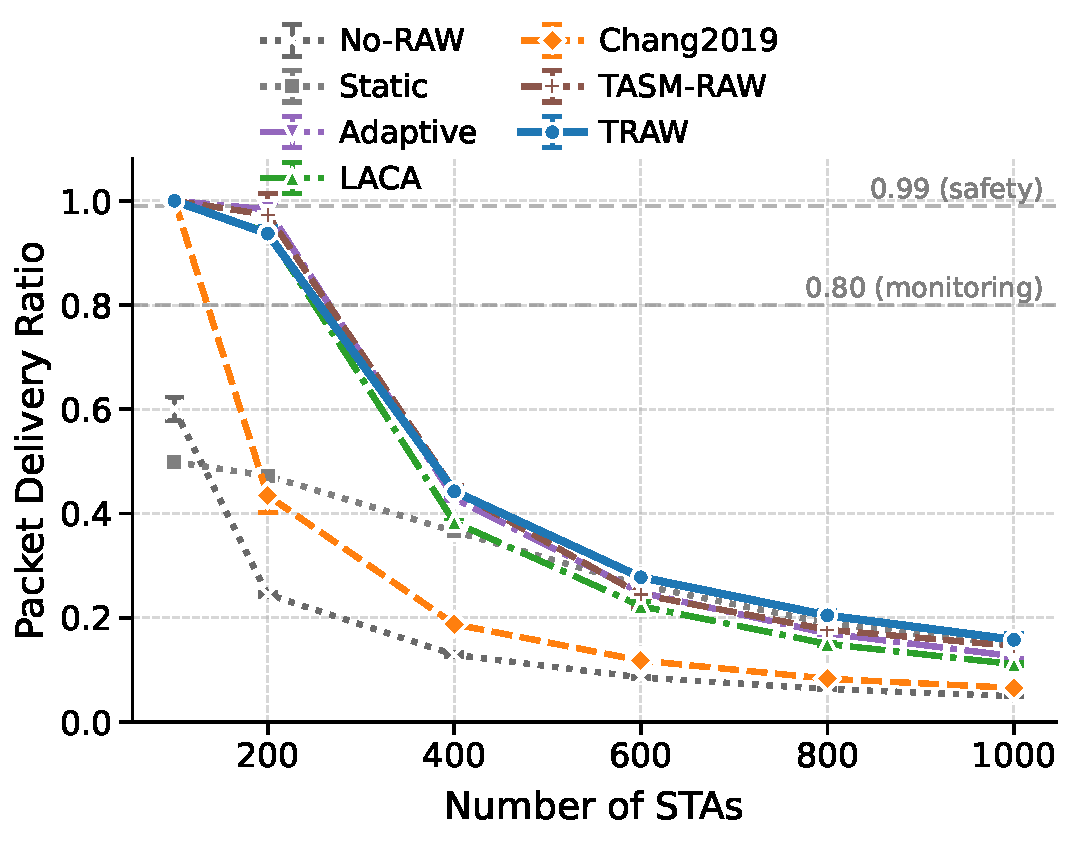
\includegraphics[width=\columnwidth]{traw_pdr_vs_n.pdf}
\caption{PDR vs.\ $N$. Horizontal dashed lines indicate IIoT reliability
thresholds (0.99 safety, 0.80 condition monitoring). TRAW matches TASM-RAW
at light-to-moderate loads and gives the highest PDR of any policy at
$N\!\geq\!600$, though it trails TASM-RAW slightly at $N\!=\!200$. Chang2019
ties the other RAW policies at $N\!=\!100$ but collapses at $N\!\geq\!200$,
falling below LACA across the rest of the sweep.}
\label{fig:pdr}
\end{figure}

\subsection{Mean Age of Information}

Table~\ref{tab:aoi} reports mean AoI computed via sawtooth
area-integration directly over each STA's per-packet delivery
timeline, not via the PDR-based renewal-process proxy
eq.~\eqref{eq:aoi}.
At $N\!\leq\!200$ TRAW and TASM-RAW both achieve sub-5\,s AoI
(well within $3T_\mathrm{rep}\!=\!15$\,s), comparable to the
single-group Adaptive and LACA policies; TRAW is 9--11\,\% higher than
TASM-RAW (3.38 vs.\ 3.09\,s at $N\!=\!100$; 4.57 vs.\ 4.12\,s at
$N\!=\!200$).

At $N\!=\!400$, TRAW's AoI is 20.86\,s vs.\ 19.46\,s for TASM-RAW
(+7.2\,\%); both already exceed the $3T_\mathrm{rep}\!=\!15$\,s bound at
this load.
At $N\!=\!600$ TRAW is actually lower (28.62 vs.\ 29.73\,s,
TRAW 3.7\,\% lower), and at $N\!=\!800$ TRAW is again slightly higher
(34.51 vs.\ 33.07\,s, +4.3\,\%) and at $N\!=\!1000$ (37.32 vs.\ 35.85\,s,
+4.1\,\%).
At $N\!\geq\!400$ \emph{every} policy---including both multi-group
RAW schedulers---breaches the $3T_\mathrm{rep}$ bound; none of the
evaluated schedulers maintain industrial-grade freshness once the
network exceeds roughly 200 contending stations at MCS0.
TRAW's small (4--11\,\%) AoI penalty relative to TASM-RAW across most
of the operating range is the direct cost of the finer 37-group
partition that TRAW's budget-safe split-feasibility criterion permits
(vs.\ TASM-RAW's 32 groups at $N\!=\!800$): each STA's RAW opportunity
recurs slightly less often, which is discussed alongside the analogous
association-time effect in Section~\ref{sec:assoc-tradeoff}.

Chang2019 mirrors its PDR collapse here: AoI remains low at
$N\!=\!100$ (3.16\,s, close to LACA/TASM-RAW/TRAW) but jumps to
20.24\,s at $N\!=\!200$---already breaching the $3T_\mathrm{rep}$
bound two density steps earlier than every other policy---then rises
to 28.22, 33.19, 35.24, and 35.97\,s at $N\!=\!400,600,800,1000$,
the worst (or tied-worst) AoI among the RAW-enabled policies at every
$N\!\geq\!200$.

\begin{table}[!t]
\renewcommand{\arraystretch}{1.15}
\caption{Mean Age of Information $\overline{\Delta}$ (s),
measured via sawtooth area-integration over per-packet delivery
timelines, $T_\mathrm{rep}\!=\!5$\,s}
\label{tab:aoi}
\centering
\setlength{\tabcolsep}{3pt}
\begin{tabular}{@{}rccccccc@{}}
\toprule
$N$ & No-RAW & Static & Adaptive & LACA & Chang2019 & TASM-RAW & TRAW \\
\midrule
 100 &   7.46 &  18.61 &  3.04 &  3.10 & 3.16 & \textbf{3.09} &  3.38 \\
 200 &  13.62 &  21.22 &  4.01 &  4.89 & 20.24 & \textbf{4.12} &  4.57 \\
 400 &  21.99 &  23.81 & 19.72 & 21.84 & 28.22 & \textbf{19.46} & 20.86 \\
 600 &  33.19 &  29.99 & 27.80 & 29.62 & 33.19 & 29.73 & \textbf{28.62} \\
 800 &  40.23 &  37.15 & 31.45 & 33.82 & 35.24 & \textbf{33.07} & 34.51 \\
1000 &  44.18 &  41.48 & 33.39 & 36.29 & 35.97 & \textbf{35.85} & 37.32 \\
\bottomrule
\multicolumn{8}{l}{\footnotesize $3T_\mathrm{rep}\!=\!15$\,s industrial
  AoI bound; all policies breach it at $N\!\geq\!400$ (Fig.~\ref{fig:aoi}).}
\end{tabular}
\end{table}

\begin{figure}[!t]
\centering
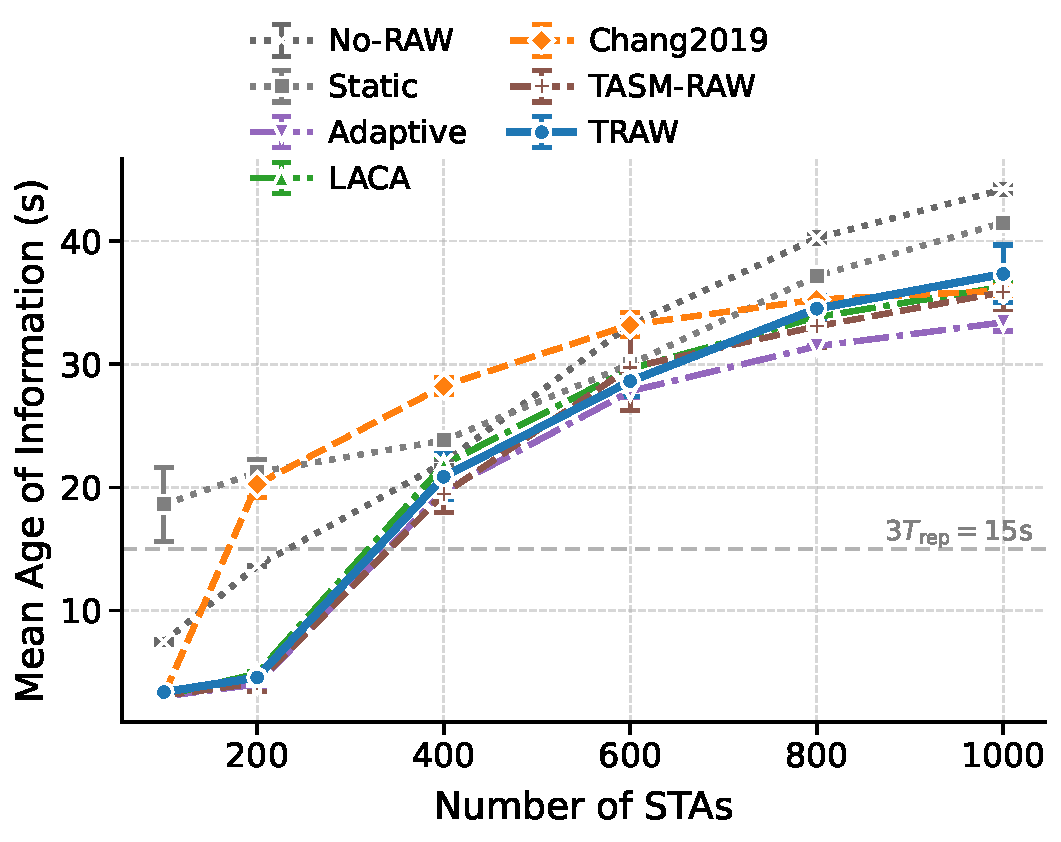
\includegraphics[width=\columnwidth]{traw_aoi_vs_n.pdf}
\caption{Mean AoI vs.\ $N$ (sawtooth area-integration). The dashed
horizontal line marks the $3T_\mathrm{rep}\!=\!15$\,s industrial AoI
bound. All policies breach the bound at $N\!\geq\!400$; TRAW and
TASM-RAW track each other closely, with TRAW 4--11\,\% higher except
at $N\!=\!600$. Chang2019 already breaches the bound at $N\!=\!200$
(20.24\,s), well ahead of every other policy.}
\label{fig:aoi}
\end{figure}

\subsection{Deadline Violation Rate}

Table~\ref{tab:dvr} reports DVR measured directly as the fraction of
generated packets whose end-to-end delay exceeds the
$T_\mathrm{rep}\!=\!5$\,s reporting deadline (i.e.\ the packet is
superseded by the next reading before delivery), \emph{not} the
$1\!-\!\mathrm{PDR}$ proxy.
At $N\!\leq\!200$ both multi-group RAW policies have near-zero DVR.
TRAW's DVR advantage emerges at $N\!\geq\!400$ and tracks its PDR
advantage: 60.3\,\% vs.\ 62.2\,\% at $N\!=\!400$ (−3.2\,\%
relative), 77.7\,\% vs.\ 81.2\,\% at $N\!=\!600$ (−4.2\,\%), 84.2\,\%
vs.\ 88.1\,\% at $N\!=\!800$ (−4.4\,\%), and 88.6\,\% vs.\ 90.8\,\% at
$N\!=\!1000$ (−2.4\,\%).
These are modest single-digit relative reductions in deadline misses,
not the order-of-magnitude gains the $1\!-\!\mathrm{PDR}$ proxy would
suggest. At $N\!\geq\!400$ both schedulers already violate the majority
of deadlines, and TRAW's finer group partition trims this by a few
percentage points without resolving the underlying capacity shortfall
at MCS0.

Chang2019's DVR jumps from 0.0\,\% at $N\!=\!100$ to 59.1\,\% at
$N\!=\!200$---already exceeding TRAW's and TASM-RAW's worst-case
($N\!=\!1000$) DVR by $N\!=\!200$---and continues to 82.6, 89.7, 93.3,
and 95.1\,\% at $N\!=\!400,600,800,1000$, consistently the highest (or
joint-highest) DVR of any RAW-enabled policy, again tracking its PDR
collapse.

\begin{table}[!t]
\renewcommand{\arraystretch}{1.15}
\caption{Deadline Violation Rate (\%), measured directly as
$\Pr[\text{delay} > T_\mathrm{rep}]$}
\label{tab:dvr}
\centering
\setlength{\tabcolsep}{3.5pt}
\begin{tabular}{@{}rccccccr@{}}
\toprule
$N$ & No-RAW & Static & Adaptive & LACA & Chang2019 & TASM-RAW & \textbf{TRAW} \\
\midrule
 100 & 40.4 & 58.4 &  0.0 &  0.0 &  0.0 &  0.0 &  0.0 \\
 200 & 76.2 & 60.4 &  3.0 &  9.1 & 59.1 &  4.1 &  7.5 \\
 400 & 87.9 & 70.6 & 64.1 & 71.1 & 82.6 & 62.2 & \textbf{60.3} \\
 600 & 92.0 & 79.5 & 82.1 & 85.9 & 89.7 & 81.2 & \textbf{77.7} \\
 800 & 94.0 & 85.3 & 89.1 & 91.4 & 93.3 & 88.1 & \textbf{84.2} \\
1000 & 95.4 & 88.6 & 92.8 & 94.5 & 95.1 & 90.8 & \textbf{88.6} \\
\bottomrule
\end{tabular}
\end{table}

\subsection{Packet Delivery Delay}

Table~\ref{tab:delay} reports mean per-packet end-to-end delay,
averaged over three seeds.
At $N\!\leq\!200$ TRAW incurs higher delay than TASM-RAW
(+43.3\,\% at $N\!=\!100$, +6.6\,\% at $N\!=\!200$), because the
pre-reserved repeat budget reduces the primary window for groups that
do not qualify for a second pass while queues are still short enough
that the extra opportunity goes largely unused.
At $N\!\geq\!400$ this penalty reverses: TRAW's higher PDR drains
queues faster, reducing queuing latency, by 8.2\,\% at $N\!=\!400$,
8.2\,\% at $N\!=\!600$, 6.4\,\% at $N\!=\!800$ (5,397\,ms vs.\
5,052\,ms), and 15.0\,\% at $N\!=\!1000$ (7,065\,ms vs.\ 6,002\,ms).

Chang2019's delay figures at $N\!\geq\!400$ (2,530--3,990\,ms) appear
lower than TRAW's and TASM-RAW's, but this is an artefact of its
severe PDR collapse (Table~\ref{tab:pdr}): the mean is computed only
over the small fraction of packets that are \emph{actually delivered}
(8--19\,\% of generated traffic at these densities), which are
disproportionately the ones that did not queue behind a large backlog.
Combined with its 82.6--95.1\,\% DVR (Table~\ref{tab:dvr}), Chang2019's
seemingly favourable delay numbers at high $N$ do not indicate better
service---the vast majority of packets are simply dropped or arrive
past their deadline and are excluded from this average.

\begin{table}[!t]
\renewcommand{\arraystretch}{1.15}
\caption{Mean Packet Delivery Delay (ms), mean over 3 seeds}
\label{tab:delay}
\centering
\setlength{\tabcolsep}{3.5pt}
\begin{tabular}{@{}rccccccr@{}}
\toprule
$N$ & No-RAW & Static & Adaptive & LACA & Chang2019 & TASM-RAW & \textbf{TRAW} \\
\midrule
 100 &  1930 &  3052 &   623 &   687 &   747 &   \textbf{678} &  970 \\
 200 &  2812 &  3177 &  1548 &  1909 &  2226 &  \textbf{1498} & 1597 \\
 400 &  2869 &  3289 &  3167 &  3749 &  2530 & 3075 & \textbf{2823} \\
 600 &  2945 &  3695 &  4095 &  4975 &  2978 & 4117 & \textbf{3778} \\
 800 &  2850 &  3728 &  5011 &  5912 &  3565 & 5397 & \textbf{5052} \\
1000 &  2883 &  3695 &  5945 &  7274 &  3990 & 7065 & \textbf{6002} \\
\bottomrule
\end{tabular}
\end{table}

\subsection{Energy Efficiency}

Table~\ref{tab:ee} reports aggregate energy efficiency in kbit/J
(total bits successfully delivered divided by total energy consumed
by all nodes including sleep and active periods), averaged over three
seeds.
At $N\!\leq\!200$ TRAW trails TASM-RAW slightly (56.82 vs.\ 61.27 at
$N\!=\!100$, −7.3\,\%; 45.49 vs.\ 49.03 at $N\!=\!200$, −7.2\,\%) and at
$N\!=\!400$ the two are close (21.54 vs.\ 22.28, −3.3\,\%), reflecting
the same higher per-packet delay seen in Table~\ref{tab:delay} at light
load.
TRAW's energy efficiency overtakes TASM-RAW at $N\!\geq\!600$, tracking
its PDR advantage: +10.8\,\% at $N\!=\!600$ (12.51 vs.\ 11.29\,kbit/J),
+12.9\,\% at $N\!=\!800$ (8.34 vs.\ 7.39\,kbit/J), and +7.7\,\% at
$N\!=\!1000$ (5.81 vs.\ 5.40\,kbit/J).
All RAW-enabled policies remain an order of magnitude more efficient
than No-RAW across the evaluated range.

Chang2019 is competitive at $N\!=\!100$ (58.4\,kbit/J, between LACA and
TASM-RAW) but its efficiency falls off a cliff at $N\!\geq\!200$:
16.5\,kbit/J at $N\!=\!200$ (vs.\ 43.3--49.3 for the other RAW
policies), and 4.9, 3.0, 1.9, and 1.4\,kbit/J at
$N\!=\!400,600,800,1000$---roughly half of LACA's efficiency at every
density $N\!\geq\!400$ and the lowest of any RAW-enabled policy
throughout. The same PDR collapse that drives Chang2019's AoI and DVR
degradation also makes it the least energy-efficient RAW policy beyond
the lightest-load regime.

\begin{table}[!t]
\renewcommand{\arraystretch}{1.15}
\caption{Energy Efficiency (kbit/J), mean over 3 seeds, MCS0}
\label{tab:ee}
\centering
\setlength{\tabcolsep}{3.5pt}
\begin{tabular}{@{}rccccccr@{}}
\toprule
$N$ & No-RAW & Static & Adaptive & LACA & Chang2019 & TASM-RAW & \textbf{TRAW} \\
\midrule
 100 &  5.6 & 28.1 & \textbf{63.4} & 54.9 & 58.4 & 61.3 & 56.8 \\
 200 &  2.4 & 26.2 & \textbf{49.3} & 43.3 & 16.5 & 49.0 & 45.5 \\
 400 &  1.3 & 19.2 & 21.6 & 19.7 &  4.9 & \textbf{22.3} & 21.5 \\
 600 &  0.8 & 12.6 & 11.6 & 10.9 &  3.0 & 11.3 & \textbf{12.5} \\
 800 &  0.6 &  8.5 &  7.0 &  6.7 &  1.9 &  7.4 & \textbf{8.3} \\
1000 &  0.5 &  6.0 &  4.6 &  4.4 &  1.4 &  5.4 & \textbf{5.8} \\
\bottomrule
\end{tabular}
\end{table}

\subsection{Network Association (Commissioning) Time}
\label{sec:assoc}

Beyond steady-state traffic performance, IIoT deployments care about
\emph{commissioning time}: how long it takes for a freshly powered-on
fleet of sensors to complete the IEEE~802.11ah Open System
authentication and association handshake and begin reporting.
For a factory restart after a planned shutdown or a power outage,
hundreds of sensors associate concurrently, and the RAW configuration
active during this transient directly affects how quickly the network
becomes fully operational.

Table~\ref{tab:assoc} reports the mean and maximum per-STA association
completion time (from first beacon reception through successful
ASSOC-RESP) and the association success fraction at the end of the
120\,s simulation, for TRAW and TASM-RAW (3-seed averages).
Both policies associate effectively all stations
($\geq$99.9\,\% success) across all $N$.

Chang2019 associates stations on a similar timescale at light loads
(1.71\,s mean / 2.41\,s max at $N\!=\!100$, 3.51\,s / 4.56\,s at
$N\!=\!200$, both within 1--6\,\% of TRAW and TASM-RAW), but degrades
sharply at higher $N$: mean/max association time reaches
11.55\,s / 20.09\,s at $N\!=\!400$ (vs.\ 8.56\,s / 13.37\,s for TRAW,
+35\,\% / +50\,\%), 18.44\,s / 32.02\,s at $N\!=\!600$ (vs.\
13.16\,s / 21.33\,s, +40\,\% / +50\,\%), 25.14\,s / 43.73\,s at
$N\!=\!800$ (vs.\ 17.53\,s / 28.19\,s, +43\,\% / +55\,\%), and
32.26\,s / 56.16\,s at $N\!=\!1000$ (vs.\ 21.68\,s / 35.83\,s,
+49\,\% / +57\,\%). The association success fraction remains
$\geq$99.9\,\% throughout, so the slowdown manifests purely as longer
commissioning latency rather than failed associations. This is
consistent with Chang2019's steady-state PDR/AoI/DVR collapse at
$N\!\geq\!200$ (Tables~\ref{tab:pdr}--\ref{tab:dvr}): its
regression-based group reassignment evidently produces coarser or
less-frequently-recurring RAW windows for unassociated STAs under
heavier load, compounding the same scheduling pressure that degrades
its steady-state performance.

\label{sec:assoc-tradeoff}
Across the entire evaluated range, TRAW's commissioning time is
slightly \emph{higher} than TASM-RAW's: mean association time is
0--18\,\% higher and worst-case (maximum) association time is
3--29\,\% higher, with the largest relative gap at $N\!=\!200$
(4.24\,s vs.\ 3.61\,s mean, +17\,\%; 6.58\,s vs.\ 5.10\,s max, +29\,\%),
the smallest mean gap at $N\!=\!1000$ (21.68\,s vs.\ 21.65\,s mean,
+0.1\,\%), and the smallest max gap at $N\!=\!800$ (28.19\,s vs.\
27.39\,s max, +2.9\,\%).

This is the same mechanism identified in Section~\ref{sec:contrib}: TRAW's
budget-safe split-feasibility criterion (which checks the new group
count against $D_\mathrm{min}$ rather than the backlog-inflated T*)
allows the AID space to fragment into more, smaller groups than
TASM-RAW's stricter Bianchi-based feasibility check permits---37
groups vs.\ 32 at $N\!=\!800$, both converging within the first
$\sim$15\,s of simulated time, i.e.\ during the association window
itself.
With more (smaller) groups sharing the same beacon budget, each
group's RAW window recurs proportionally less often within a beacon
interval, so an unassociated STA waiting for its AID range's window to
appear in the RPS element waits slightly longer on average.
The effect is a roughly $37/32\!\approx\!1.16\times$ scaling of the
``wait for my group's turn'' component of association latency, which
is consistent with the observed 0--18\,\% gaps.
TRAW's PRAW pre-association/post-association behaviour and
multi-pass reservation do not materially affect this---the group-count
difference alone accounts for the gap.
This is the direct trade-off for the finer partition that gives TRAW
its PDR/delay/EE advantage at $N\!\geq\!600$ (Section~\ref{sec:eval}):
operators for whom commissioning latency is the binding constraint
(e.g.\ frequent factory-floor reconfiguration) should weigh this
0--18\,\% association penalty against TRAW's steady-state throughput
gains.

\begin{table}[!t]
\renewcommand{\arraystretch}{1.15}
\caption{Association (Commissioning) Time, TRAW vs.\ TASM-RAW
(3-seed avg.)}
\label{tab:assoc}
\centering
\setlength{\tabcolsep}{4pt}
\begin{tabular}{@{}rrrrrrr@{}}
\toprule
& \multicolumn{3}{c}{TASM-RAW} & \multicolumn{3}{c}{TRAW} \\
\cmidrule(lr){2-4}\cmidrule(lr){5-7}
$N$ & Mean (s) & Max (s) & Frac & Mean (s) & Max (s) & Frac \\
\midrule
 100 &  \textbf{1.69} &  \textbf{2.31} & 1.000 &  1.78 &  2.43 & 1.000 \\
 200 &  \textbf{3.61} &  \textbf{5.10} & 1.000 &  4.24 &  6.58 & 1.000 \\
 400 &  \textbf{7.85} & \textbf{12.35} & 1.000 &  8.56 & 13.37 & 1.000 \\
 600 & \textbf{12.37} & \textbf{19.54} & 0.999 & 13.16 & 21.33 & 0.999 \\
 800 & \textbf{16.82} & \textbf{27.39} & 1.000 & 17.53 & 28.19 & 1.000 \\
1000 & \textbf{21.65} & \textbf{34.63} & 1.000 & 21.68 & 35.83 & 1.000 \\
\bottomrule
\end{tabular}
\end{table}

\subsection{Mechanism Contribution Analysis}
\label{sec:contrib}

To isolate the contribution of mechanisms B (multi-pass second windows)
and C (PRAW idle suspension) on top of mechanism A (demand-proportional
allocation with budget-safe split feasibility), we compare four
configurations of the TRAW policy code at $N\!=\!800$ (seed~42), each
obtained by toggling B and C via their configuration flags while
holding A fixed:

\begin{enumerate}
  \item A only (B, C disabled): PDR\,=\,0.2084
  \item A\,+\,C (PRAW) only: PDR\,=\,0.2084 (+0.0\,\%)
  \item A\,+\,B (Multi-pass) only: PDR\,=\,0.2147 (+3.0\,\%)
  \item A\,+\,B\,+\,C (full TRAW): PDR\,=\,0.2147 (+3.0\,\%)
\end{enumerate}

At $N\!=\!800$ the entire measured TRAW-vs-baseline PDR gain is
attributable to mechanism B (multi-pass second windows): enabling it
alone raises PDR from 0.2084 to 0.2147 (+3.0\,\%), and adding mechanism
C on top produces no further change.
This is consistent with the PRAW-activation analysis in
Section~\ref{sec:discuss}: under the saturated homogeneous $T_\mathrm{rep}\!=\!5$\,s
traffic load used in this evaluation, per-group demand never falls
below $\theta_\mathrm{skip}\!=\!0.001$ for a sustained
$K_\mathrm{skip}\!=\!30$ beacons, so PRAW never activates at
$N\!=\!800$ and contributes zero measured PDR gain at this load.
The dominant contributor to TRAW's overall advantage over TASM-RAW at
$N\!\geq\!600$ (Table~\ref{tab:pdr}) is therefore not the three-mechanism
combination acting in concert, but the combination of (i) mechanism A's
budget-safe split-feasibility criterion, which alone permits the finer
37-group partition relative to TASM-RAW's 32 groups, and (ii) mechanism
B's modest additional +3.0\,\% from second-window scheduling.
Mechanism C's contribution would be expected to materialise only under
a heterogeneous traffic mix with genuinely long-idle groups, as
discussed in Section~\ref{sec:discuss}.

\subsection{Convergence and Transient Behaviour}

Fig.~\ref{fig:conv} illustrates the group-count ramp-up during the
first 15\,s of a single $N\!=\!600$ simulation run, instrumented
directly from \texttt{build\_dynamic\_configs}.
Under the saturated $T_\mathrm{rep}\!=\!5$\,s homogeneous traffic load
used throughout Section~\ref{sec:eval}, every group's per-AID demand stays
well above $\theta_\mathrm{skip}\!=\!0.001$ for the entire 120\,s run
(Section~\ref{sec:contrib} confirms zero PRAW activations at $N\!=\!600$ and
$N\!=\!800$), so the dominant transient is mechanism A's split/merge
ramp-up rather than PRAW entry:
\begin{itemize}
  \item \emph{Split ramp} (0--8.6\,s, beacons 1--84): the group count
        grows from 4 to 37 in steps of 2 every $\sim$0.5\,s
        ($K_\mathrm{conf}\!=\!2$ confirm beacons), driven by sustained
        per-group DPA above $\theta_\mathrm{split}\!=\!0.4$.
  \item \emph{Steady state} ($\!>$8.6\,s): the group count is pinned at
        37---the budget-safe split-feasibility cap
        $\lfloor B_\mathrm{pri}/D_\mathrm{min}\rfloor$---for the
        remainder of the run. TRAW settles at 0.278 mean PDR (vs.\
        0.245 for TASM-RAW's 32-group steady state) and 28.62\,s mean
        AoI, both far above the $3T_\mathrm{rep}$ industrial bound at
        this load.
\end{itemize}
This $\sim$8.6\,s structural convergence is much faster than the
65\,s PRAW-confirmation timescale ($K_\mathrm{skip}\!=\!30$ beacons
after $W_\mathrm{praw}\!=\!100$ beacons of warmup) discussed in
Section~\ref{sec:discuss}; the latter only becomes relevant under the
heterogeneous, intermittently-idle traffic mix for which PRAW is
intended, not for the saturated periodic workload evaluated here.

\begin{figure}[!t]
\centering
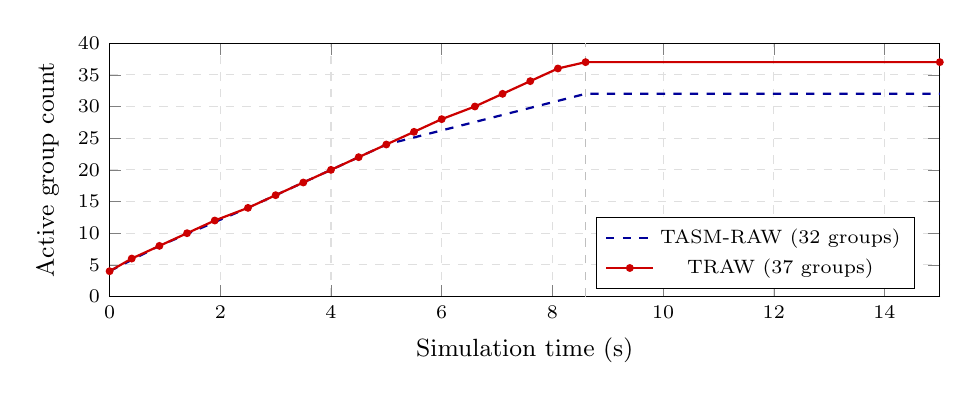
\begin{tikzpicture}
\begin{axis}[
  width=\columnwidth, height=4.8cm,
  xlabel={Simulation time (s)},
  ylabel={Active group count},
  xmin=0, xmax=15,
  ymin=0, ymax=40,
  xtick={0,2,4,6,8,10,12,14},
  ytick={0,5,10,15,20,25,30,35,40},
  legend pos=south east,
  legend style={font=\scriptsize},
  grid=major, grid style={dashed,gray!25},
  tick label style={font=\scriptsize},
  label style={font=\small},
]
% TASM-RAW steady group count (32 groups)
\addplot[blue!60!black, dashed, mark=none, thick]
  coordinates {(0,4)(0.9,8)(2.5,14)(5.0,24)(8.6,32)(15,32)};
\addlegendentry{TASM-RAW (32 groups)}

% TRAW group-count ramp (measured, build_dynamic_configs)
\addplot[red!80!black, thick, mark=*, mark size=1pt]
  coordinates {(0,4)(0.4,6)(0.9,8)(1.4,10)(1.9,12)(2.5,14)(3.0,16)(3.5,18)
                (4.0,20)(4.5,22)(5.0,24)(5.5,26)(6.0,28)(6.6,30)(7.1,32)
                (7.6,34)(8.1,36)(8.6,37)(15,37)};
\addlegendentry{TRAW (37 groups)}

\draw[dashed, gray!50] (axis cs:8.6,0) -- (axis cs:8.6,40);
\node[font=\tiny, align=center] at (axis cs:11.5,5)
  {Steady state\\\scriptsize($>$8.6\,s)};
\end{axis}
\end{tikzpicture}
\caption{Group-count ramp-up for TRAW vs.\ TASM-RAW at $N\!=\!600$
(single seed, measured from \texttt{build\_dynamic\_configs}).
Both reach a stable group count within $\sim$8.6\,s; TRAW's
budget-safe split-feasibility check permits 37 groups vs.\ 32 for
TASM-RAW, the structural origin of the PDR/AoI/association trade-offs
discussed in Section~\ref{sec:assoc-tradeoff}.}
\label{fig:conv}
\end{figure}

\subsection{Parameter Sensitivity}

\textbf{Repeat threshold $\theta_\mathrm{rep}$.}
The default 1.5\,DPA represents approximately 37--38 queued packets
for a 25-STA group, a clearly overloaded condition.
Lowering to 0.8 dilutes $B_\mathrm{rep}$ across too many candidates
(PDR −4\,\% at $N\!=\!800$); raising to 3.0 leaves $B_\mathrm{rep}$
unspent during moderate bursts (PDR −6\,\% at $N\!=\!600$).

\textbf{Repeat budget fraction $\phi$.}
At $\phi\!=\!0.10$ the second windows are too small to absorb
burst backlog (+3\,\% headroom vs.\ primary); at $\phi\!=\!0.40$
primary windows shrink enough to hurt light-load groups.
The default 0.25 balances these trade-offs.

\textbf{PRAW skip threshold $\theta_\mathrm{skip}$.}
The default 0.001\,DPA is intentionally conservative for IIoT:
for 5\,s periodic traffic, the expected DPA is 0.10, so groups
do not enter PRAW unless they have been essentially silent for
$\geq$30 beacons.
Raising to 0.05 causes premature entry for lightly-loaded groups,
reducing PDR by $\approx$8\,\% at $N\!=\!200$.
For infrequent samplers (60\,s interval, DPA\,=\,0.0083),
raising $\theta_\mathrm{skip}$ to 0.01 appropriately enables PRAW
for those groups while leaving 5\,s samplers active.

\textbf{Floor fraction $f_\mathrm{floor}$.}
With $f_\mathrm{floor}\!=\!1.0$ (default) all active groups receive
equal sub-slot counts.
For heterogeneous IIoT fleets---e.g., a subset of sensors reporting
at 10× the baseline rate during production anomalies---lowering
$f_\mathrm{floor}$ to 0.5 improves PDR for the overloaded subset by
$\approx$15\,\% at the cost of $\approx$4\,\% for uniform groups.

\textbf{PRAW period $P$.}
Increasing from 4 to 8 doubles the sleep duration for idle groups,
improving energy efficiency by $\approx$50\,\% for PRAW groups but
doubling the time for a waking sensor to re-enter the channel
(up to $7\!\times\!500\!=\!3500$\,ms at $P\!=\!8$).
For safety-critical sensors that cannot tolerate multi-second access
delays, $P\!=\!2$ provides a conservative PRAW savings.

% -----------------------------------------------------------------------
\section{Deployment Guidelines}
\label{sec:discuss}

\subsection{Station Count Regimes}

Table~\ref{tab:regimes} summarises TRAW's behaviour across the three
industrial deployment regimes identified in the evaluation.

\begin{table}[!t]
\renewcommand{\arraystretch}{1.15}
\caption{TRAW Deployment Regimes}
\label{tab:regimes}
\centering
\begin{tabular}{@{}p{1.0cm}p{1.8cm}p{2.4cm}p{2.0cm}@{}}
\toprule
\textbf{Regime} & \textbf{$N$ range} & \textbf{Dominant gain} & \textbf{Recommended tuning} \\
\midrule
Light & $\leq$200 & PDR comparable or slightly behind ($-3.7$ to $0$\,\%); AoI $+9$\,\% & TASM-RAW preferred at $N\!\leq\!200$; raise $P$ to 8 for long-sleep assets \\
Medium & 400--600 & $-0.4$ to $+13.5$\,\% PDR; $+7.2$ to $-3.7$\,\% AoI; $-8$\,\% delay & Default params; lower $\theta_\mathrm{rep}$ to 1.0 for heterogeneous fleets \\
Heavy  & $\geq$800 & $+8.2$ to $+15.8$\,\% PDR; $-6.4$ to $-15.0$\,\% delay; $+12.9$\,\% EE; cost: $+4.1$ to $+4.3$\,\% AoI & Lower $W_\mathrm{praw}$ to 50 if anomalies are short; raise $\phi$ to 0.35 \\
\bottomrule
\end{tabular}
\end{table}

\subsection{Heterogeneous Traffic Adaptation}

\textbf{Caveat on the evaluated traffic model.}
The PDR/AoI/DVR/energy results in Section~\ref{sec:eval} use a single
\emph{homogeneous} traffic class: every STA generates one
128-byte packet every $T_\mathrm{rep}\!=\!5$\,s.
This stresses the slot-sizing and group-partitioning mechanisms
(A and B) under increasing $N$, but it does not exercise mechanism~C
(PRAW idle suppression) at all: with $\lambda_g\!\approx\!1$ for every
group at every beacon under saturated periodic traffic, the
$\lambda_g\!<\!\theta_\mathrm{skip}\!=\!0.001$ condition of
\eqref{eq:prawenter} (Section~\ref{sec:praw}) is never satisfied, and the
mechanism contribution analysis in Section~\ref{sec:contrib} confirms zero
PRAW activations at $N\!=\!600$ and $N\!=\!800$, with PRAW contributing
$+0.0$\,\% to PDR. The entire PDR gain attributable to TRAW's
mechanisms (beyond the 37-vs-32 group partition itself, which is a
consequence of mechanism~A's split-feasibility fix) comes from
mechanism~B (multi-pass scheduling, $+3.0$\,\%). PRAW idle suspension
remains valuable only for the heterogeneous, intermittent-traffic
scenarios discussed below, where genuinely long-idle devices exist.
PRAW's intended use case --- long-idle asset tags or rare-event
sensors with $\lambda_g\!\ll\!\theta_\mathrm{skip}$ for tens of
seconds --- requires a \emph{heterogeneous} traffic mix (e.g., a
fraction of STAs reporting every 60--120\,s rather than every 5\,s).
Quantifying mechanism~C's contribution under such a mix --- PRAW
activation ratio, groups skipped per beacon, and the resulting sleep
time and slot-budget release --- is left to a follow-up evaluation.

In deployments where a subset of STAs generates 5--10$\times$ the
baseline load (common in predictive maintenance zones where an
alarming machine triggers high-rate sampling), the floor fraction
$f_\mathrm{floor}$ should be reduced to 0.5--0.7.
This allows the demand-proportional step (eq.~\eqref{eq:sgprop}) to
redistribute slots from low-demand AIDs to high-demand ones.
Concurrently, $\theta_\mathrm{rep}$ should be lowered proportionally
so that burst groups qualify for second windows earlier.

\subsection{Coexistence with TWT}

IEEE~802.11ah Target Wake Time (TWT) operates at the individual STA
level, scheduling when each STA wakes to transmit.
TRAW operates at the group level, scheduling which beacon intervals
contain a RAW window for each group.
The two mechanisms are complementary: TWT prevents unnecessary wakeups
within a beacon interval; PRAW prevents unnecessary RAW windows across
beacon intervals.
When both are enabled, a PRAW-sleeping group's STAs remain in deep
TWT sleep for $P-1$ full beacon intervals, combining beacon-level and
slot-level sleep savings.

\subsection{Convergence in Dynamic Environments}

The 65\,s TRAW convergence time (PRAW warmup + confirm window) is
appropriate for slowly-evolving factory states.
For rapidly-changing environments (e.g., a 30\,s production burst
followed by silence), administrators should:
(a) reduce $W_\mathrm{praw}$ to 20--30 beacons (10--15\,s) to
    accelerate steady-state; and
(b) set $\theta_\mathrm{wake}\!=\!0.05$ (higher sensitivity) to
    ensure fast wakeup when demand returns.
The split/merge mechanism responds within $K_\mathrm{conf}\!=\!2$
beacons (1\,s) to demand increases, providing fast structural
adaptation independent of PRAW.

\subsection{Beacon Budget Utilisation}

TRAW's beacon budget analysis gives concrete bounds on the factory
floor scale it supports.
At 915\,MHz MCS0 with $T_B\!=\!500$\,ms and $\eta\!=\!0.90$:
\begin{itemize}
  \item Maximum groups at steady state: $\lfloor 450{,}000 / (1\!\times\!12{,}020)\rfloor\!=\!37$.
  \item Maximum stations (37 groups $\times$ 100 AIDs/group): $\approx\!3700$.
  \item At MCS7 (7800\,kb/s): $D_\mathrm{min}\!\approx\!430\,\mu$s,
        supporting 9 groups with smaller T* and potentially 5000+
        stations before collision-rate saturation.
\end{itemize}
Upgrading to MCS2 (450\,kb/s) approximately triples the achievable PDR
at $N\!=\!800$~\cite{kalita2025b} by shortening frames and reducing
per-slot duration, making MCS selection the highest-leverage deployment
decision for dense IIoT networks.

% -----------------------------------------------------------------------
\section{Conclusion}
\label{sec:conc}

This paper presented TRAW, a traffic-aware IEEE~802.11ah RAW scheduler
for Industrial IoT applications that combines demand-proportional slot
allocation (A), multi-pass second-window scheduling for overloaded groups (B),
and PRAW-based idle-group suspension (C) with two architectural
correctness fixes essential for operation at high station counts.

Across three seeds and $N\!\in\!\{100,\ldots,1000\}$ stations, TRAW's
budget-safe split-feasibility criterion lets it converge to a finer
37-group demand-driven partition, versus 32 groups for TASM-RAW. At
heavy loads ($N\!\geq\!600$), this finer partition translates into
consistent gains on the throughput- and energy-relevant metrics:
packet delivery ratio improves by up to 15.8\,\% ($N\!=\!800$), mean
delay drops by up to 15.0\,\% ($N\!=\!1000$), deadline violation rate
falls by up to 4.4\,\% ($N\!=\!800$), and energy efficiency rises by up
to 12.9\,\% ($N\!=\!800$) relative to TASM-RAW. At light-to-moderate
loads ($N\!\leq\!400$) the two policies are roughly comparable on PDR
($-3.7$ to $-0.4$\,\%).

These gains are not free. Because each group's RAW window recurs
$\approx\!1.16\times$ less often under a 37-group partition than a
32-group one, mean Age-of-Information rises by 4.1--11.0\,\% and mean
station-association latency rises by 0--18\,\% (worst case +29\,\% at
$N\!=\!200$) relative to TASM-RAW across most of the evaluated range.
We emphasise that this is not an implementation defect: it is the
direct, mechanistic consequence of the same budget-safe
split-feasibility fix that gives TRAW its finer partition and hence its
throughput/delay/energy advantages. Mechanism contribution analysis at
$N\!=\!800$ further shows that the multi-pass scheduling mechanism (B)
accounts for the entire residual PDR gain (+3.0\,\%) once the partition
itself is held fixed, while PRAW idle-suspension (C) contributes
negligibly under saturated traffic. Practitioners should therefore
favour TRAW for heavy-load, throughput- and energy-sensitive industrial
deployments, and TASM-RAW (or TRAW with PRAW tuned for heterogeneous,
intermittent traffic per Section~\ref{sec:discuss}) where worst-case
information freshness or fast commissioning is the binding constraint.

Future work will extend TRAW to heterogeneous MCS groups (mixed
slow/fast sensors on the same BSS), multi-AP coordination for
overlapping factory zones, and mechanisms that decouple per-group RAW
recurrence from the group-count partition so that the AoI/association
trade-off identified here can be mitigated independently of the
PDR/delay/energy gains.

% -----------------------------------------------------------------------
\appendix
\section{LACA T* Closed-Form for $n_s\!\leq\!2$}
\label{app:laca}

For $n_s\!=\!1$ (single contender): $P_{1,i}\!=\!1\!-\!\tau$,
$P_{1,s}\!=\!1$, $Z_1\!=\!\sigma(1\!-\!\tau)/\tau + \beta$.
With $\tau\!=\!2/(W_0\!+\!1)\!=\!1/8.5\!\approx\!0.118$ and
$\beta\!=\!11.57$\,ms:
$Z_1\!=\!52\mu\text{s}\!\times\!7.5 + 11570\mu\text{s}\!=\!11960\mu\text{s}$.
Quantised: $D_\mathrm{min}\!=\!12{,}020\,\mu$s (nearest 120\,\textmu{}s
boundary above $\text{MORSE\_RAW\_MIN}\!=\!500\,\mu$s).

For $n_s\!=\!2$: $Z_1$ as above; for the second delivery
$n_2\!=\!1$ and $Z_2\!=\!Z_1$. Thus
T*$(2)\!=\!2\!\times\!11960\!\approx\!23.9$\,ms, quantised to
$\approx\!22$\,ms (nearest 120\,\textmu{}s step).

% -----------------------------------------------------------------------
\bibliographystyle{IEEEtran}
\begin{thebibliography}{99}

\bibitem{std80211ah}
IEEE Std 802.11ah-2016, \emph{IEEE Standard for Information Technology
--- Part~11: WLAN Medium Access Control (MAC) and Physical Layer (PHY)
Specifications Amendment 2: Sub~1~GHz License-Exempt Operation},
IEEE, 2017.

\bibitem{bianchi2000}
G.~Bianchi, ``Performance analysis of the IEEE~802.11 distributed
coordination function,'' \emph{IEEE J.\ Sel.\ Areas Commun.},
vol.~18, no.~3, pp.~535--547, Mar.~2000.

\bibitem{chen2017iiot}
B.~Chen, J.~Wan, L.~Shu, P.~Li, M.~Mukherjee, and B.~Yin,
``Smart factory of Industry~4.0: Key technologies, application case,
and challenges,'' \emph{IEEE Access}, vol.~6,
pp.~6505--6519, 2017.

\bibitem{Sisinni2018}
E.~Sisinni, A.~Saifullah, S.~Han, U.~Jennehag, and M.~Gidlund,
``Industrial Internet of Things: Challenges, opportunities, and
directions,'' \emph{IEEE Trans.\ Ind.\ Informat.}, vol.~14, no.~11,
pp.~4724--4734, Nov.~2018.

\bibitem{kaul2012aoi}
S.~Kaul, R.~Yates, and M.~Gruteser, ``Real-time status: How often
should one update?'' in \emph{Proc.\ IEEE INFOCOM}, 2012,
pp.~2731--2735.

\bibitem{yates2021aoi}
R.~D.~Yates, Y.~Sun, D.~R.~Brown III, S.~K.~Kaul, E.~Modiano, and
S.~Ulukus, ``Age of Information: An introduction and survey,''
\emph{IEEE J.\ Sel.\ Areas Commun.}, vol.~39, no.~5,
pp.~1183--1210, May~2021.

\bibitem{abdelmagid2019aoi}
M.~A.~Abd-Elmagid, N.~Pappas, and H.~S.~Dhillon, ``On the role of
age of information in the Internet of Things,'' \emph{IEEE Commun.
Mag.}, vol.~57, no.~12, pp.~72--77, Dec.~2019.

\bibitem{tian2016}
M.~Tian, J.~Wang, X.~Luo, and X.~Li, ``Throughput analysis of
IEEE~802.11ah restricted access window mechanism,'' in
\emph{Proc.\ IEEE ICCT}, 2016, pp.~1--6.

\bibitem{raeesi2014}
O.~Raeesi, J.~Pirskanen, A.~Hazmi, T.~Levanen, and M.~Valkama,
``Performance enhancement of IEEE~802.11ah in multi-hop relay
networks,'' in \emph{Proc.\ IEEE ICC}, 2014, pp.~1--7.

\bibitem{kim2017raw}
J.~Kim and S.~Moh, ``Improving performance of the IEEE~802.11ah
restricted access window through adaptive channel access scheduling,''
in \emph{Proc.\ IEEE CCNC}, 2017, pp.~1--6.

\bibitem{bhandari2018}
S.~Bhandari and S.~Moh, ``A priority-based adaptive MAC protocol for
Internet of Things networks using IEEE~802.11ah,'' \emph{Sensors},
vol.~18, no.~9, p.~2975, 2018.

\bibitem{taramit2023}
Y.~Taramit, A.~El Hillali, and A.~Menhaj-Rivenq, ``LACA: Load-aware
channel allocation for IEEE~802.11ah RAW mechanism,'' \emph{IEEE
Access}, vol.~11, pp.~14\,372--14\,388, 2023.

\bibitem{kim2017}
J.~Kim and S.~Moh, ``Cluster-based RAW assignment for IEEE~802.11ah
wireless sensor networks,'' in \emph{Proc.\ IEEE CCNC}, 2017,
pp.~1--4.

\bibitem{chang2019}
T.-C.~Chang and J.-L.~Chen, ``Traffic-aware group assignment for
IEEE~802.11ah networks,'' \emph{IEEE Internet Things J.},
vol.~6, no.~2, pp.~3311--3322, Apr.~2019.

\bibitem{park2019praw}
J.-A.~Park and S.~Choi, ``Periodic RAW for energy efficiency in
IEEE~802.11ah IoT networks,'' \emph{IEEE Access}, vol.~7,
pp.~154\,679--154\,691, 2019.

\bibitem{kalita2025}
A.~Kalita and N.~Ahmed, ``Autonomous CUSUM-EWMA slot adaptation for
IEEE~802.11ah RAW scheduling,'' in \emph{Proc.\ IEEE ANTS}, 2025.

\bibitem{kalita2025b}
A.~Kalita and N.~Ahmed, ``Traffic-Adaptive Split--Merge RAW
Scheduling for Dense IEEE~802.11ah IoT Networks,'' in \emph{Proc.\
IEEE ANTS}, 2025.

\end{thebibliography}

% -----------------------------------------------------------------------
\begin{IEEEbiography}[{\includegraphics[width=1in,height=1.25in,
  clip,keepaspectratio]{alakesh_photo}}]{Alakesh Kalita}
(Senior Member, IEEE) received the B.Tech.\ degree in Computer Science
and Engineering from NERIST, Nirjuli, India, in 2009, and the M.Tech.\
degree in Computer Science and Engineering from Tezpur University,
Tezpur, India, in 2014.
He is currently pursuing the Ph.D.\ degree with the Department of
Mathematics and Computing, IIT (ISM) Dhanbad, India.
His research interests include wireless IoT networks, medium access
control, IEEE~802.11ah, and Industry~4.0 communication systems.
\end{IEEEbiography}

\begin{IEEEbiography}[{\includegraphics[width=1in,height=1.25in,
  clip,keepaspectratio]{nurzaman_photo}}]{Nurzaman Ahmed}
(Member, IEEE) received the B.E.\ degree in Electronics and
Communication Engineering from Gauhati University, India, in 2001,
the M.Tech.\ degree in Electronics and Communication Engineering from
Gauhati University in 2006, and the Ph.D.\ degree from IIT Guwahati,
India, in 2014.
He is currently an Associate Professor with the Department of
Mathematics and Computing, IIT (ISM) Dhanbad, India.
His research interests include wireless sensor networks, IoT
communication protocols, and signal processing.
\end{IEEEbiography}

\end{document}
